\documentclass[twoside]{book}

% Packages required by doxygen
\usepackage{fixltx2e}
\usepackage{calc}
\usepackage{doxygen}
\usepackage[export]{adjustbox} % also loads graphicx
\usepackage{graphicx}
\usepackage[utf8]{inputenc}
\usepackage{makeidx}
\usepackage{multicol}
\usepackage{multirow}
\PassOptionsToPackage{warn}{textcomp}
\usepackage{textcomp}
\usepackage[nointegrals]{wasysym}
\usepackage[table]{xcolor}

% Font selection
\usepackage[T1]{fontenc}
\usepackage[scaled=.90]{helvet}
\usepackage{courier}
\usepackage{amssymb}
\usepackage{sectsty}
\renewcommand{\familydefault}{\sfdefault}
\allsectionsfont{%
  \fontseries{bc}\selectfont%
  \color{darkgray}%
}
\renewcommand{\DoxyLabelFont}{%
  \fontseries{bc}\selectfont%
  \color{darkgray}%
}
\newcommand{\+}{\discretionary{\mbox{\scriptsize$\hookleftarrow$}}{}{}}

% Page & text layout
\usepackage{geometry}
\geometry{%
  a4paper,%
  top=2.5cm,%
  bottom=2.5cm,%
  left=2.5cm,%
  right=2.5cm%
}
\tolerance=750
\hfuzz=15pt
\hbadness=750
\setlength{\emergencystretch}{15pt}
\setlength{\parindent}{0cm}
\setlength{\parskip}{3ex plus 2ex minus 2ex}
\makeatletter
\renewcommand{\paragraph}{%
  \@startsection{paragraph}{4}{0ex}{-1.0ex}{1.0ex}{%
    \normalfont\normalsize\bfseries\SS@parafont%
  }%
}
\renewcommand{\subparagraph}{%
  \@startsection{subparagraph}{5}{0ex}{-1.0ex}{1.0ex}{%
    \normalfont\normalsize\bfseries\SS@subparafont%
  }%
}
\makeatother

% Headers & footers
\usepackage{fancyhdr}
\pagestyle{fancyplain}
\fancyhead[LE]{\fancyplain{}{\bfseries\thepage}}
\fancyhead[CE]{\fancyplain{}{}}
\fancyhead[RE]{\fancyplain{}{\bfseries\leftmark}}
\fancyhead[LO]{\fancyplain{}{\bfseries\rightmark}}
\fancyhead[CO]{\fancyplain{}{}}
\fancyhead[RO]{\fancyplain{}{\bfseries\thepage}}
\fancyfoot[LE]{\fancyplain{}{}}
\fancyfoot[CE]{\fancyplain{}{}}
\fancyfoot[RE]{\fancyplain{}{\bfseries\scriptsize Generated by Doxygen }}
\fancyfoot[LO]{\fancyplain{}{\bfseries\scriptsize Generated by Doxygen }}
\fancyfoot[CO]{\fancyplain{}{}}
\fancyfoot[RO]{\fancyplain{}{}}
\renewcommand{\footrulewidth}{0.4pt}
\renewcommand{\chaptermark}[1]{%
  \markboth{#1}{}%
}
\renewcommand{\sectionmark}[1]{%
  \markright{\thesection\ #1}%
}

% Indices & bibliography
\usepackage{natbib}
\usepackage[titles]{tocloft}
\setcounter{tocdepth}{3}
\setcounter{secnumdepth}{5}
\makeindex

% Hyperlinks (required, but should be loaded last)
\usepackage{ifpdf}
\ifpdf
  \usepackage[pdftex,pagebackref=true]{hyperref}
\else
  \usepackage[ps2pdf,pagebackref=true]{hyperref}
\fi
\hypersetup{%
  colorlinks=true,%
  linkcolor=blue,%
  citecolor=blue,%
  unicode%
}

% Custom commands
\newcommand{\clearemptydoublepage}{%
  \newpage{\pagestyle{empty}\cleardoublepage}%
}

\usepackage{caption}
\captionsetup{labelsep=space,justification=centering,font={bf},singlelinecheck=off,skip=4pt,position=top}

%===== C O N T E N T S =====

\begin{document}

% Titlepage & ToC
\hypersetup{pageanchor=false,
             bookmarksnumbered=true,
             pdfencoding=unicode
            }
\pagenumbering{roman}
\begin{titlepage}
\vspace*{7cm}
\begin{center}%
{\Large My Project }\\
\vspace*{1cm}
{\large Generated by Doxygen 1.8.11}\\
\end{center}
\end{titlepage}
\clearemptydoublepage
\tableofcontents
\clearemptydoublepage
\pagenumbering{arabic}
\hypersetup{pageanchor=true}

%--- Begin generated contents ---
\chapter{Research Track 1 -\/ final assignment}
\label{md_README}
\hypertarget{md_README}{}
This package is the result of my work on the final assignment of Reaserch Track module 1 course.

\subsection*{General information}

Once runned , this package will provide an interface and nodes to control a robot in a Gazebo simulation, allowing the user to chose between different behaviours for the robot to navigate the environment. In order to be able to work with this package, also the package {\bfseries movebase} and {\bfseries gmapping} are needed.

\subsection*{How to run}

In the {\itshape launch} folder of this package there are 4 launch files, in order to set everything up please run in order \+:


\begin{DoxyCode}
1 roslaunch final\_assignment gmapping.launch
\end{DoxyCode}
 
\begin{DoxyCode}
1 roslaunch final ssignment movebase.launch
\end{DoxyCode}
 
\begin{DoxyCode}
1 roslaunch final assignment main.launch
\end{DoxyCode}


At this point the interface should be online

\subsection*{Additional documentation}

To find the complete documentation for this project go in {\itshape docs/html} folder and open {\bfseries index.\+html} 
\chapter{Namespace Index}
\section{Namespace List}
Here is a list of all namespaces with brief descriptions\+:\begin{DoxyCompactList}
\item\contentsline{section}{\hyperlink{namespacebig__brain}{big\+\_\+brain} }{\pageref{namespacebig__brain}}{}
\item\contentsline{section}{\hyperlink{namespacebig__user__interface}{big\+\_\+user\+\_\+interface} }{\pageref{namespacebig__user__interface}}{}
\item\contentsline{section}{\hyperlink{namespacebug__algo}{bug\+\_\+algo} }{\pageref{namespacebug__algo}}{}
\item\contentsline{section}{\hyperlink{namespacefinal__assignment}{final\+\_\+assignment} \\*This node is in charge of monitoring the state of the robot, and activate the corresping services and behaviour }{\pageref{namespacefinal__assignment}}{}
\item\contentsline{section}{\hyperlink{namespacego__to__point__service__bug}{go\+\_\+to\+\_\+point\+\_\+service\+\_\+bug} }{\pageref{namespacego__to__point__service__bug}}{}
\item\contentsline{section}{\hyperlink{namespaceuser__interface}{user\+\_\+interface} }{\pageref{namespaceuser__interface}}{}
\item\contentsline{section}{\hyperlink{namespacewall__follower__service}{wall\+\_\+follower\+\_\+service} }{\pageref{namespacewall__follower__service}}{}
\item\contentsline{section}{\hyperlink{namespacewall__follower__service__bug}{wall\+\_\+follower\+\_\+service\+\_\+bug} }{\pageref{namespacewall__follower__service__bug}}{}
\end{DoxyCompactList}

\chapter{File Index}
\section{File List}
Here is a list of all files with brief descriptions\+:\begin{DoxyCompactList}
\item\contentsline{section}{scripts/\hyperlink{big__brain_8py}{big\+\_\+brain.\+py} }{\pageref{big__brain_8py}}{}
\item\contentsline{section}{scripts/\hyperlink{big__user__interface_8py}{big\+\_\+user\+\_\+interface.\+py} }{\pageref{big__user__interface_8py}}{}
\item\contentsline{section}{scripts/\hyperlink{bug__algo_8py}{bug\+\_\+algo.\+py} }{\pageref{bug__algo_8py}}{}
\item\contentsline{section}{scripts/\hyperlink{go__to__point__service__bug_8py}{go\+\_\+to\+\_\+point\+\_\+service\+\_\+bug.\+py} }{\pageref{go__to__point__service__bug_8py}}{}
\item\contentsline{section}{scripts/\hyperlink{user__interface_8py}{user\+\_\+interface.\+py} }{\pageref{user__interface_8py}}{}
\item\contentsline{section}{scripts/\hyperlink{wall__follower__service_8py}{wall\+\_\+follower\+\_\+service.\+py} }{\pageref{wall__follower__service_8py}}{}
\item\contentsline{section}{scripts/\hyperlink{wall__follower__service__bug_8py}{wall\+\_\+follower\+\_\+service\+\_\+bug.\+py} }{\pageref{wall__follower__service__bug_8py}}{}
\end{DoxyCompactList}

\chapter{Namespace Documentation}
\hypertarget{namespacebig__brain}{}\section{big\+\_\+brain Namespace Reference}
\label{namespacebig__brain}\index{big\+\_\+brain@{big\+\_\+brain}}
\subsection*{Functions}
\begin{DoxyCompactItemize}
\item 
def \hyperlink{namespacebig__brain_a815c120863ef1a5db7bf743bc9bb6f54}{clbk\+\_\+odom} (msg)
\begin{DoxyCompactList}\small\item\em Callback for keeping track of robot pose. \end{DoxyCompactList}\item 
def \hyperlink{namespacebig__brain_adfc26e0690fd9fe893e09be5400a8b7d}{distance} ()
\begin{DoxyCompactList}\small\item\em Function for computing the distance from the robot actual position to the desired position. \end{DoxyCompactList}\item 
def \hyperlink{namespacebig__brain_a4f091a106e4ba678afd9bc2df4f2789b}{new\+\_\+goal} ()
\begin{DoxyCompactList}\small\item\em Function for setting a new target with a Move\+Base\+Action\+Goal msg on topic /movebase/goal. \end{DoxyCompactList}\item 
def \hyperlink{namespacebig__brain_a108d0111d106a89cde8da1c2f494ab3c}{change\+\_\+state} (state)
\begin{DoxyCompactList}\small\item\em Function for changing the state of the robot. \end{DoxyCompactList}\item 
def \hyperlink{namespacebig__brain_a06516fa995f70f4013ee893ae15c5cea}{main} ()
\begin{DoxyCompactList}\small\item\em Main function. \end{DoxyCompactList}\end{DoxyCompactItemize}
\subsection*{Variables}
\begin{DoxyCompactItemize}
\item 
\hyperlink{namespacebig__brain_a9f12d1c3982160fe18122c7a2c4aa860}{twist\+\_\+pub} = None
\begin{DoxyCompactList}\small\item\em Publisher that publishes on /cmd\+\_\+vel to stop the robot when entering in state of \textquotesingle{}stop\textquotesingle{}. \end{DoxyCompactList}\item 
\hyperlink{namespacebig__brain_a757b56b184f850f2599be2279ac94777}{mvgoal\+\_\+pub} = None
\begin{DoxyCompactList}\small\item\em Publisher that publish a Move\+Base\+Action\+Goal msg on /move\+\_\+base/goal to make the robot reach the goal. \end{DoxyCompactList}\item 
\hyperlink{namespacebig__brain_acbbe2e86c0b737f0caaff69ce22b4aa8}{mvcancel\+\_\+pub} = None
\begin{DoxyCompactList}\small\item\em Publisher that publish a Goal\+ID msg on /move\+\_\+base/cancel to cancel a previous goal. \end{DoxyCompactList}\item 
\hyperlink{namespacebig__brain_a954157b5770aed51dc667611f39855b0}{srv\+\_\+client\+\_\+wall\+\_\+follower\+\_\+} = None
\begin{DoxyCompactList}\small\item\em Client for activating the service for wall following behaviour. \end{DoxyCompactList}\item 
\hyperlink{namespacebig__brain_a946162ac048b8df1f02003b37bd96812}{srv\+\_\+client\+\_\+user\+\_\+interface\+\_\+assignment\+\_\+} = None
\begin{DoxyCompactList}\small\item\em Client for activating the service calling the user main user interface. \end{DoxyCompactList}\item 
\hyperlink{namespacebig__brain_a60d3104e99b35d213a90529c7bc5a573}{srv\+\_\+client\+\_\+bug\+\_\+algorithm\+\_\+} = None
\begin{DoxyCompactList}\small\item\em C\+Lient for activating the bug navigation behaviour. \end{DoxyCompactList}\item 
\hyperlink{namespacebig__brain_a463bcdb8c7ed9954756492cdce9a43e2}{position\+\_\+} = Point()
\begin{DoxyCompactList}\small\item\em Variable containing position of the robot. \end{DoxyCompactList}\item 
\hyperlink{namespacebig__brain_a5f0f2fbee791fd60caa7a9dcf6ca1e00}{regions\+\_\+} = None
\begin{DoxyCompactList}\small\item\em Variables for controlling laser data. \end{DoxyCompactList}\item 
int \hyperlink{namespacebig__brain_ac43f9e8255d9b336a4f3ebe4dc3d2246}{change\+\_\+} = 0
\begin{DoxyCompactList}\small\item\em Variable for checking if a new state has been issued. \end{DoxyCompactList}\item 
list \hyperlink{namespacebig__brain_ab730e09c9bd7f5c7a1c09a8ea55a9029}{state\+\_\+desc\+\_\+} = \mbox{[}\textquotesingle{}random target\textquotesingle{}, \textquotesingle{}get target\textquotesingle{}, \textquotesingle{}wall fallowing\textquotesingle{},\textquotesingle{}stop\textquotesingle{},\textquotesingle{}bug\textquotesingle{}\mbox{]}
\begin{DoxyCompactList}\small\item\em States of the robot definiton. \end{DoxyCompactList}\item 
int \hyperlink{namespacebig__brain_a95db081b16847592a7981a7205e66358}{state\+\_\+} = 0
\begin{DoxyCompactList}\small\item\em Variable cointaining the actual state of the robot. \end{DoxyCompactList}\item 
int \hyperlink{namespacebig__brain_a28f405a0651539e59bd455a35ab07a3c}{newstate\+\_\+} = 0
\begin{DoxyCompactList}\small\item\em Variable containing the new state of the robot. \end{DoxyCompactList}\item 
int \hyperlink{namespacebig__brain_a82350019fe3047e74222abd0d6b07c14}{user\+\_\+} = 0
\begin{DoxyCompactList}\small\item\em Variable to control the different user interface when the behaviour is switched to bug. \end{DoxyCompactList}\end{DoxyCompactItemize}


\subsection{Function Documentation}
\index{big\+\_\+brain@{big\+\_\+brain}!change\+\_\+state@{change\+\_\+state}}
\index{change\+\_\+state@{change\+\_\+state}!big\+\_\+brain@{big\+\_\+brain}}
\subsubsection[{\texorpdfstring{change\+\_\+state(state)}{change_state(state)}}]{\setlength{\rightskip}{0pt plus 5cm}def big\+\_\+brain.\+change\+\_\+state (
\begin{DoxyParamCaption}
\item[{}]{state}
\end{DoxyParamCaption}
)}\hypertarget{namespacebig__brain_a108d0111d106a89cde8da1c2f494ab3c}{}\label{namespacebig__brain_a108d0111d106a89cde8da1c2f494ab3c}


Function for changing the state of the robot. 

This function changes the state of the robot activating the various services and the respectfull operations set only the request for service for first behaviour to True Set wall follow and bug algorithm behaviour to false call new goal for setting the new target 

Here is the call graph for this function\+:\nopagebreak
\begin{figure}[H]
\begin{center}
\leavevmode
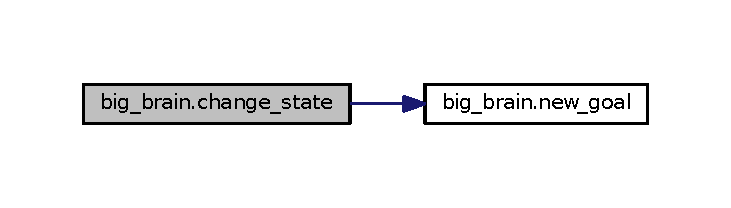
\includegraphics[width=350pt]{namespacebig__brain_a108d0111d106a89cde8da1c2f494ab3c_cgraph}
\end{center}
\end{figure}




Here is the caller graph for this function\+:\nopagebreak
\begin{figure}[H]
\begin{center}
\leavevmode
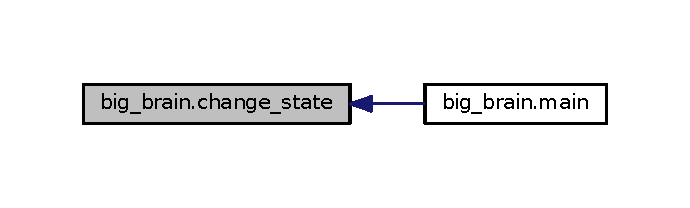
\includegraphics[width=331pt]{namespacebig__brain_a108d0111d106a89cde8da1c2f494ab3c_icgraph}
\end{center}
\end{figure}


\index{big\+\_\+brain@{big\+\_\+brain}!clbk\+\_\+odom@{clbk\+\_\+odom}}
\index{clbk\+\_\+odom@{clbk\+\_\+odom}!big\+\_\+brain@{big\+\_\+brain}}
\subsubsection[{\texorpdfstring{clbk\+\_\+odom(msg)}{clbk_odom(msg)}}]{\setlength{\rightskip}{0pt plus 5cm}def big\+\_\+brain.\+clbk\+\_\+odom (
\begin{DoxyParamCaption}
\item[{}]{msg}
\end{DoxyParamCaption}
)}\hypertarget{namespacebig__brain_a815c120863ef1a5db7bf743bc9bb6f54}{}\label{namespacebig__brain_a815c120863ef1a5db7bf743bc9bb6f54}


Callback for keeping track of robot pose. 

Callback for subscriber of /odom for checking robot pose. 
\begin{DoxyParams}{Parameters}
{\em msg} & geometry\+\_\+msgs/\+Odometry \\
\hline
\end{DoxyParams}
\index{big\+\_\+brain@{big\+\_\+brain}!distance@{distance}}
\index{distance@{distance}!big\+\_\+brain@{big\+\_\+brain}}
\subsubsection[{\texorpdfstring{distance()}{distance()}}]{\setlength{\rightskip}{0pt plus 5cm}def big\+\_\+brain.\+distance (
\begin{DoxyParamCaption}
{}
\end{DoxyParamCaption}
)}\hypertarget{namespacebig__brain_adfc26e0690fd9fe893e09be5400a8b7d}{}\label{namespacebig__brain_adfc26e0690fd9fe893e09be5400a8b7d}


Function for computing the distance from the robot actual position to the desired position. 



Here is the caller graph for this function\+:\nopagebreak
\begin{figure}[H]
\begin{center}
\leavevmode
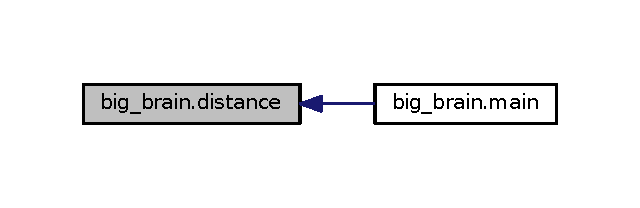
\includegraphics[width=307pt]{namespacebig__brain_adfc26e0690fd9fe893e09be5400a8b7d_icgraph}
\end{center}
\end{figure}


\index{big\+\_\+brain@{big\+\_\+brain}!main@{main}}
\index{main@{main}!big\+\_\+brain@{big\+\_\+brain}}
\subsubsection[{\texorpdfstring{main()}{main()}}]{\setlength{\rightskip}{0pt plus 5cm}def big\+\_\+brain.\+main (
\begin{DoxyParamCaption}
{}
\end{DoxyParamCaption}
)}\hypertarget{namespacebig__brain_a06516fa995f70f4013ee893ae15c5cea}{}\label{namespacebig__brain_a06516fa995f70f4013ee893ae15c5cea}


Main function. 

initializes necessary variables, works as a state machine 

Here is the call graph for this function\+:\nopagebreak
\begin{figure}[H]
\begin{center}
\leavevmode
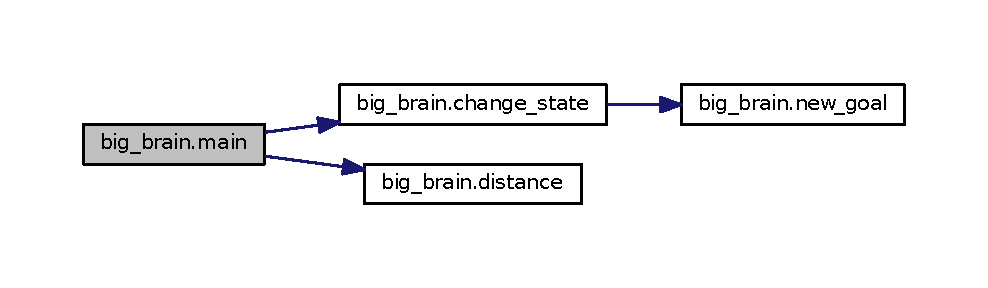
\includegraphics[width=350pt]{namespacebig__brain_a06516fa995f70f4013ee893ae15c5cea_cgraph}
\end{center}
\end{figure}


\index{big\+\_\+brain@{big\+\_\+brain}!new\+\_\+goal@{new\+\_\+goal}}
\index{new\+\_\+goal@{new\+\_\+goal}!big\+\_\+brain@{big\+\_\+brain}}
\subsubsection[{\texorpdfstring{new\+\_\+goal()}{new_goal()}}]{\setlength{\rightskip}{0pt plus 5cm}def big\+\_\+brain.\+new\+\_\+goal (
\begin{DoxyParamCaption}
{}
\end{DoxyParamCaption}
)}\hypertarget{namespacebig__brain_a4f091a106e4ba678afd9bc2df4f2789b}{}\label{namespacebig__brain_a4f091a106e4ba678afd9bc2df4f2789b}


Function for setting a new target with a Move\+Base\+Action\+Goal msg on topic /movebase/goal. 



Here is the caller graph for this function\+:\nopagebreak
\begin{figure}[H]
\begin{center}
\leavevmode
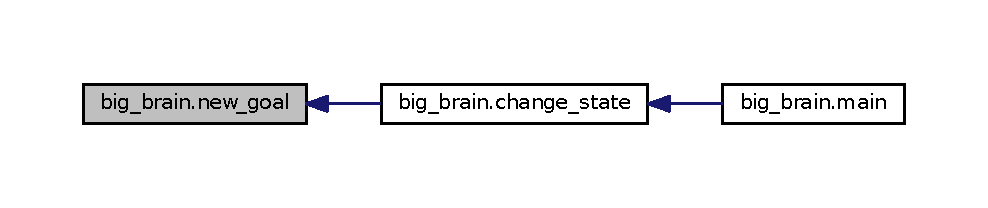
\includegraphics[width=350pt]{namespacebig__brain_a4f091a106e4ba678afd9bc2df4f2789b_icgraph}
\end{center}
\end{figure}




\subsection{Variable Documentation}
\index{big\+\_\+brain@{big\+\_\+brain}!change\+\_\+@{change\+\_\+}}
\index{change\+\_\+@{change\+\_\+}!big\+\_\+brain@{big\+\_\+brain}}
\subsubsection[{\texorpdfstring{change\+\_\+}{change_}}]{\setlength{\rightskip}{0pt plus 5cm}int big\+\_\+brain.\+change\+\_\+ = 0}\hypertarget{namespacebig__brain_ac43f9e8255d9b336a4f3ebe4dc3d2246}{}\label{namespacebig__brain_ac43f9e8255d9b336a4f3ebe4dc3d2246}


Variable for checking if a new state has been issued. 

\index{big\+\_\+brain@{big\+\_\+brain}!mvcancel\+\_\+pub@{mvcancel\+\_\+pub}}
\index{mvcancel\+\_\+pub@{mvcancel\+\_\+pub}!big\+\_\+brain@{big\+\_\+brain}}
\subsubsection[{\texorpdfstring{mvcancel\+\_\+pub}{mvcancel_pub}}]{\setlength{\rightskip}{0pt plus 5cm}big\+\_\+brain.\+mvcancel\+\_\+pub = None}\hypertarget{namespacebig__brain_acbbe2e86c0b737f0caaff69ce22b4aa8}{}\label{namespacebig__brain_acbbe2e86c0b737f0caaff69ce22b4aa8}


Publisher that publish a Goal\+ID msg on /move\+\_\+base/cancel to cancel a previous goal. 

\index{big\+\_\+brain@{big\+\_\+brain}!mvgoal\+\_\+pub@{mvgoal\+\_\+pub}}
\index{mvgoal\+\_\+pub@{mvgoal\+\_\+pub}!big\+\_\+brain@{big\+\_\+brain}}
\subsubsection[{\texorpdfstring{mvgoal\+\_\+pub}{mvgoal_pub}}]{\setlength{\rightskip}{0pt plus 5cm}big\+\_\+brain.\+mvgoal\+\_\+pub = None}\hypertarget{namespacebig__brain_a757b56b184f850f2599be2279ac94777}{}\label{namespacebig__brain_a757b56b184f850f2599be2279ac94777}


Publisher that publish a Move\+Base\+Action\+Goal msg on /move\+\_\+base/goal to make the robot reach the goal. 

\index{big\+\_\+brain@{big\+\_\+brain}!newstate\+\_\+@{newstate\+\_\+}}
\index{newstate\+\_\+@{newstate\+\_\+}!big\+\_\+brain@{big\+\_\+brain}}
\subsubsection[{\texorpdfstring{newstate\+\_\+}{newstate_}}]{\setlength{\rightskip}{0pt plus 5cm}int big\+\_\+brain.\+newstate\+\_\+ = 0}\hypertarget{namespacebig__brain_a28f405a0651539e59bd455a35ab07a3c}{}\label{namespacebig__brain_a28f405a0651539e59bd455a35ab07a3c}


Variable containing the new state of the robot. 

\index{big\+\_\+brain@{big\+\_\+brain}!position\+\_\+@{position\+\_\+}}
\index{position\+\_\+@{position\+\_\+}!big\+\_\+brain@{big\+\_\+brain}}
\subsubsection[{\texorpdfstring{position\+\_\+}{position_}}]{\setlength{\rightskip}{0pt plus 5cm}big\+\_\+brain.\+position\+\_\+ = Point()}\hypertarget{namespacebig__brain_a463bcdb8c7ed9954756492cdce9a43e2}{}\label{namespacebig__brain_a463bcdb8c7ed9954756492cdce9a43e2}


Variable containing position of the robot. 

\index{big\+\_\+brain@{big\+\_\+brain}!regions\+\_\+@{regions\+\_\+}}
\index{regions\+\_\+@{regions\+\_\+}!big\+\_\+brain@{big\+\_\+brain}}
\subsubsection[{\texorpdfstring{regions\+\_\+}{regions_}}]{\setlength{\rightskip}{0pt plus 5cm}big\+\_\+brain.\+regions\+\_\+ = None}\hypertarget{namespacebig__brain_a5f0f2fbee791fd60caa7a9dcf6ca1e00}{}\label{namespacebig__brain_a5f0f2fbee791fd60caa7a9dcf6ca1e00}


Variables for controlling laser data. 

\index{big\+\_\+brain@{big\+\_\+brain}!srv\+\_\+client\+\_\+bug\+\_\+algorithm\+\_\+@{srv\+\_\+client\+\_\+bug\+\_\+algorithm\+\_\+}}
\index{srv\+\_\+client\+\_\+bug\+\_\+algorithm\+\_\+@{srv\+\_\+client\+\_\+bug\+\_\+algorithm\+\_\+}!big\+\_\+brain@{big\+\_\+brain}}
\subsubsection[{\texorpdfstring{srv\+\_\+client\+\_\+bug\+\_\+algorithm\+\_\+}{srv_client_bug_algorithm_}}]{\setlength{\rightskip}{0pt plus 5cm}big\+\_\+brain.\+srv\+\_\+client\+\_\+bug\+\_\+algorithm\+\_\+ = None}\hypertarget{namespacebig__brain_a60d3104e99b35d213a90529c7bc5a573}{}\label{namespacebig__brain_a60d3104e99b35d213a90529c7bc5a573}


C\+Lient for activating the bug navigation behaviour. 

\index{big\+\_\+brain@{big\+\_\+brain}!srv\+\_\+client\+\_\+user\+\_\+interface\+\_\+assignment\+\_\+@{srv\+\_\+client\+\_\+user\+\_\+interface\+\_\+assignment\+\_\+}}
\index{srv\+\_\+client\+\_\+user\+\_\+interface\+\_\+assignment\+\_\+@{srv\+\_\+client\+\_\+user\+\_\+interface\+\_\+assignment\+\_\+}!big\+\_\+brain@{big\+\_\+brain}}
\subsubsection[{\texorpdfstring{srv\+\_\+client\+\_\+user\+\_\+interface\+\_\+assignment\+\_\+}{srv_client_user_interface_assignment_}}]{\setlength{\rightskip}{0pt plus 5cm}big\+\_\+brain.\+srv\+\_\+client\+\_\+user\+\_\+interface\+\_\+assignment\+\_\+ = None}\hypertarget{namespacebig__brain_a946162ac048b8df1f02003b37bd96812}{}\label{namespacebig__brain_a946162ac048b8df1f02003b37bd96812}


Client for activating the service calling the user main user interface. 

\index{big\+\_\+brain@{big\+\_\+brain}!srv\+\_\+client\+\_\+wall\+\_\+follower\+\_\+@{srv\+\_\+client\+\_\+wall\+\_\+follower\+\_\+}}
\index{srv\+\_\+client\+\_\+wall\+\_\+follower\+\_\+@{srv\+\_\+client\+\_\+wall\+\_\+follower\+\_\+}!big\+\_\+brain@{big\+\_\+brain}}
\subsubsection[{\texorpdfstring{srv\+\_\+client\+\_\+wall\+\_\+follower\+\_\+}{srv_client_wall_follower_}}]{\setlength{\rightskip}{0pt plus 5cm}big\+\_\+brain.\+srv\+\_\+client\+\_\+wall\+\_\+follower\+\_\+ = None}\hypertarget{namespacebig__brain_a954157b5770aed51dc667611f39855b0}{}\label{namespacebig__brain_a954157b5770aed51dc667611f39855b0}


Client for activating the service for wall following behaviour. 

\index{big\+\_\+brain@{big\+\_\+brain}!state\+\_\+@{state\+\_\+}}
\index{state\+\_\+@{state\+\_\+}!big\+\_\+brain@{big\+\_\+brain}}
\subsubsection[{\texorpdfstring{state\+\_\+}{state_}}]{\setlength{\rightskip}{0pt plus 5cm}int big\+\_\+brain.\+state\+\_\+ = 0}\hypertarget{namespacebig__brain_a95db081b16847592a7981a7205e66358}{}\label{namespacebig__brain_a95db081b16847592a7981a7205e66358}


Variable cointaining the actual state of the robot. 

\index{big\+\_\+brain@{big\+\_\+brain}!state\+\_\+desc\+\_\+@{state\+\_\+desc\+\_\+}}
\index{state\+\_\+desc\+\_\+@{state\+\_\+desc\+\_\+}!big\+\_\+brain@{big\+\_\+brain}}
\subsubsection[{\texorpdfstring{state\+\_\+desc\+\_\+}{state_desc_}}]{\setlength{\rightskip}{0pt plus 5cm}list big\+\_\+brain.\+state\+\_\+desc\+\_\+ = \mbox{[}\textquotesingle{}random target\textquotesingle{}, \textquotesingle{}get target\textquotesingle{}, \textquotesingle{}wall fallowing\textquotesingle{},\textquotesingle{}stop\textquotesingle{},\textquotesingle{}bug\textquotesingle{}\mbox{]}}\hypertarget{namespacebig__brain_ab730e09c9bd7f5c7a1c09a8ea55a9029}{}\label{namespacebig__brain_ab730e09c9bd7f5c7a1c09a8ea55a9029}


States of the robot definiton. 

\index{big\+\_\+brain@{big\+\_\+brain}!twist\+\_\+pub@{twist\+\_\+pub}}
\index{twist\+\_\+pub@{twist\+\_\+pub}!big\+\_\+brain@{big\+\_\+brain}}
\subsubsection[{\texorpdfstring{twist\+\_\+pub}{twist_pub}}]{\setlength{\rightskip}{0pt plus 5cm}big\+\_\+brain.\+twist\+\_\+pub = None}\hypertarget{namespacebig__brain_a9f12d1c3982160fe18122c7a2c4aa860}{}\label{namespacebig__brain_a9f12d1c3982160fe18122c7a2c4aa860}


Publisher that publishes on /cmd\+\_\+vel to stop the robot when entering in state of \textquotesingle{}stop\textquotesingle{}. 

\index{big\+\_\+brain@{big\+\_\+brain}!user\+\_\+@{user\+\_\+}}
\index{user\+\_\+@{user\+\_\+}!big\+\_\+brain@{big\+\_\+brain}}
\subsubsection[{\texorpdfstring{user\+\_\+}{user_}}]{\setlength{\rightskip}{0pt plus 5cm}int big\+\_\+brain.\+user\+\_\+ = 0}\hypertarget{namespacebig__brain_a82350019fe3047e74222abd0d6b07c14}{}\label{namespacebig__brain_a82350019fe3047e74222abd0d6b07c14}


Variable to control the different user interface when the behaviour is switched to bug. 


\hypertarget{namespacebig__user__interface}{}\section{big\+\_\+user\+\_\+interface Namespace Reference}
\label{namespacebig__user__interface}\index{big\+\_\+user\+\_\+interface@{big\+\_\+user\+\_\+interface}}
\subsection*{Functions}
\begin{DoxyCompactItemize}
\item 
def \hyperlink{namespacebig__user__interface_a76119123837eb23b6351dfa51682c794}{random\+\_\+trgt} (minimum, maximum)
\begin{DoxyCompactList}\small\item\em F\+Unction for setting a desired position. \end{DoxyCompactList}\item 
def \hyperlink{namespacebig__user__interface_a681a3a84ae63765bf0d5e1ea19486d57}{assignment} (req)
\begin{DoxyCompactList}\small\item\em Function to assign a new behaviour to the robot. \end{DoxyCompactList}\item 
def \hyperlink{namespacebig__user__interface_ad2af43c69156cede1e27c973c8193d9c}{main} ()
\begin{DoxyCompactList}\small\item\em Main function. \end{DoxyCompactList}\end{DoxyCompactItemize}


\subsection{Function Documentation}
\index{big\+\_\+user\+\_\+interface@{big\+\_\+user\+\_\+interface}!assignment@{assignment}}
\index{assignment@{assignment}!big\+\_\+user\+\_\+interface@{big\+\_\+user\+\_\+interface}}
\subsubsection[{\texorpdfstring{assignment(req)}{assignment(req)}}]{\setlength{\rightskip}{0pt plus 5cm}def big\+\_\+user\+\_\+interface.\+assignment (
\begin{DoxyParamCaption}
\item[{}]{req}
\end{DoxyParamCaption}
)}\hypertarget{namespacebig__user__interface_a681a3a84ae63765bf0d5e1ea19486d57}{}\label{namespacebig__user__interface_a681a3a84ae63765bf0d5e1ea19486d57}


Function to assign a new behaviour to the robot. 

Asks the user to insert a new desired behaviour and sets the parameters for the next change in state 

Here is the call graph for this function\+:\nopagebreak
\begin{figure}[H]
\begin{center}
\leavevmode
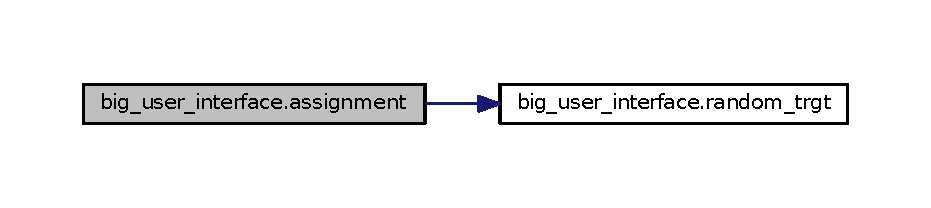
\includegraphics[width=350pt]{namespacebig__user__interface_a681a3a84ae63765bf0d5e1ea19486d57_cgraph}
\end{center}
\end{figure}


\index{big\+\_\+user\+\_\+interface@{big\+\_\+user\+\_\+interface}!main@{main}}
\index{main@{main}!big\+\_\+user\+\_\+interface@{big\+\_\+user\+\_\+interface}}
\subsubsection[{\texorpdfstring{main()}{main()}}]{\setlength{\rightskip}{0pt plus 5cm}def big\+\_\+user\+\_\+interface.\+main (
\begin{DoxyParamCaption}
{}
\end{DoxyParamCaption}
)}\hypertarget{namespacebig__user__interface_ad2af43c69156cede1e27c973c8193d9c}{}\label{namespacebig__user__interface_ad2af43c69156cede1e27c973c8193d9c}


Main function. 

Initializes the service server for user\+\_\+interface\+\_\+assignments \index{big\+\_\+user\+\_\+interface@{big\+\_\+user\+\_\+interface}!random\+\_\+trgt@{random\+\_\+trgt}}
\index{random\+\_\+trgt@{random\+\_\+trgt}!big\+\_\+user\+\_\+interface@{big\+\_\+user\+\_\+interface}}
\subsubsection[{\texorpdfstring{random\+\_\+trgt(minimum, maximum)}{random_trgt(minimum, maximum)}}]{\setlength{\rightskip}{0pt plus 5cm}def big\+\_\+user\+\_\+interface.\+random\+\_\+trgt (
\begin{DoxyParamCaption}
\item[{}]{minimum, }
\item[{}]{maximum}
\end{DoxyParamCaption}
)}\hypertarget{namespacebig__user__interface_a76119123837eb23b6351dfa51682c794}{}\label{namespacebig__user__interface_a76119123837eb23b6351dfa51682c794}


F\+Unction for setting a desired position. 

the six possible positions has been enumerated from 1 to 6 set the parameters of desired position according to the number that has been extracted. minimun and maximum are 1 and 6 for random target but since I use this function also to set the position when is the user to select one of the six, in this case minumum=maximum 
\begin{DoxyParams}{Parameters}
{\em minimum} & minimum of the range \\
\hline
{\em maximum} & maximum of the range \\
\hline
\end{DoxyParams}


Here is the caller graph for this function\+:\nopagebreak
\begin{figure}[H]
\begin{center}
\leavevmode
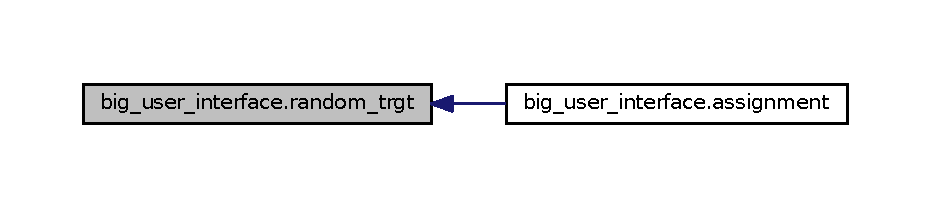
\includegraphics[width=350pt]{namespacebig__user__interface_a76119123837eb23b6351dfa51682c794_icgraph}
\end{center}
\end{figure}



\hypertarget{namespacebug__algo}{}\section{bug\+\_\+algo Namespace Reference}
\label{namespacebug__algo}\index{bug\+\_\+algo@{bug\+\_\+algo}}
\subsection*{Functions}
\begin{DoxyCompactItemize}
\item 
def \hyperlink{namespacebug__algo_a6a72a118f8a289bf80b1fe79487b273f}{clbk\+\_\+odom} (msg)
\begin{DoxyCompactList}\small\item\em Function to retrieve robot pose. \end{DoxyCompactList}\item 
def \hyperlink{namespacebug__algo_a4363ca4faa041280e958c5141bc3bde8}{clbk\+\_\+laser} (msg)
\begin{DoxyCompactList}\small\item\em Laser data callback. \end{DoxyCompactList}\item 
def \hyperlink{namespacebug__algo_afe2965502b3ec1efdb6ac2dadfb9a5de}{bug\+\_\+algorithm\+\_\+srv} (req)
\begin{DoxyCompactList}\small\item\em Function activated on service request. \end{DoxyCompactList}\item 
def \hyperlink{namespacebug__algo_aca287deda75aa8d0f790135ef47b6a16}{change\+\_\+state} (state)
\begin{DoxyCompactList}\small\item\em Change state function. \end{DoxyCompactList}\item 
def \hyperlink{namespacebug__algo_ae499da57d8d88a30b64054480fdb60c8}{normalize\+\_\+angle} (angle)
\begin{DoxyCompactList}\small\item\em Normalize angle function. \end{DoxyCompactList}\item 
def \hyperlink{namespacebug__algo_a8df2ef2049aa935d5478597523b50dcb}{main} ()
\begin{DoxyCompactList}\small\item\em Main function. \end{DoxyCompactList}\end{DoxyCompactItemize}
\subsection*{Variables}
\begin{DoxyCompactItemize}
\item 
bool \hyperlink{namespacebug__algo_a3bec537d2bfc115b0a14ee6bad41bd00}{active\+\_\+} = False
\item 
int \hyperlink{namespacebug__algo_a6ff626c7bf6a4dfec4e8508d8ae5097c}{start\+\_\+time} = 0
\item 
int \hyperlink{namespacebug__algo_af723ba0d909555b34934483c74e06818}{elapsed\+\_\+time} = 0
\item 
int \hyperlink{namespacebug__algo_af9e77fe7842316d1491ef585c7602710}{actual\+\_\+time} = 0
\item 
\hyperlink{namespacebug__algo_a17a7504f2f0f6714f6ac31a43107fc31}{pub} = None
\item 
\hyperlink{namespacebug__algo_a52e8d210b667d955534f12f59f191eb3}{srv\+\_\+client\+\_\+go\+\_\+to\+\_\+point\+\_\+} = None
\item 
\hyperlink{namespacebug__algo_afe0f6c6a1a9bc751e4bbcae499815585}{srv\+\_\+client\+\_\+wall\+\_\+follower\+\_\+} = None
\item 
\hyperlink{namespacebug__algo_a1a55011236874d9af4afcf4c3524bbf0}{srv\+\_\+client\+\_\+user\+\_\+interface\+\_\+} = None
\item 
\hyperlink{namespacebug__algo_ac9de3b470960260c4510748850446480}{srv\+\_\+client\+\_\+user\+\_\+interface\+\_\+assignment\+\_\+} = None
\item 
int \hyperlink{namespacebug__algo_a2c8d86dd369e86415dc7ff9c617033d7}{yaw\+\_\+} = 0
\item 
int \hyperlink{namespacebug__algo_a3714c955ff3cf688c84d6dc5654833d6}{yaw\+\_\+error\+\_\+allowed\+\_\+} = 5
\item 
\hyperlink{namespacebug__algo_ac0035ad008802f966f437b4787365220}{position\+\_\+} = Point()
\item 
\hyperlink{namespacebug__algo_a6bc76d9dd5213819c8287c8833f8f3bd}{desired\+\_\+position\+\_\+} = Point()
\item 
\hyperlink{namespacebug__algo_ae006850add8691db5d752b4ccb732ac1}{x}
\item 
\hyperlink{namespacebug__algo_a1e2d049a4b898c92454f0fb146a413ee}{y}
\item 
\hyperlink{namespacebug__algo_ad9944dcf5037184fbfbe3162935d2a57}{z}
\item 
\hyperlink{namespacebug__algo_a31fd6300649f8a600eb87ebed00b174f}{regions\+\_\+} = None
\item 
list \hyperlink{namespacebug__algo_a419cb7998b9a3946692fc01f5d73a25b}{state\+\_\+desc\+\_\+} = \mbox{[}\textquotesingle{}Go to point\textquotesingle{}, \textquotesingle{}wall following\textquotesingle{}, \textquotesingle{}stopped\textquotesingle{}\mbox{]}
\item 
int \hyperlink{namespacebug__algo_a5bf52a66b7821a097f6e653a2422748e}{state\+\_\+} = 0
\end{DoxyCompactItemize}


\subsection{Function Documentation}
\index{bug\+\_\+algo@{bug\+\_\+algo}!bug\+\_\+algorithm\+\_\+srv@{bug\+\_\+algorithm\+\_\+srv}}
\index{bug\+\_\+algorithm\+\_\+srv@{bug\+\_\+algorithm\+\_\+srv}!bug\+\_\+algo@{bug\+\_\+algo}}
\subsubsection[{\texorpdfstring{bug\+\_\+algorithm\+\_\+srv(req)}{bug_algorithm_srv(req)}}]{\setlength{\rightskip}{0pt plus 5cm}def bug\+\_\+algo.\+bug\+\_\+algorithm\+\_\+srv (
\begin{DoxyParamCaption}
\item[{}]{req}
\end{DoxyParamCaption}
)}\hypertarget{namespacebug__algo_afe2965502b3ec1efdb6ac2dadfb9a5de}{}\label{namespacebug__algo_afe2965502b3ec1efdb6ac2dadfb9a5de}


Function activated on service request. 


\begin{DoxyParams}{Parameters}
{\em req} & is the request of the service \\
\hline
\end{DoxyParams}


Here is the call graph for this function\+:\nopagebreak
\begin{figure}[H]
\begin{center}
\leavevmode
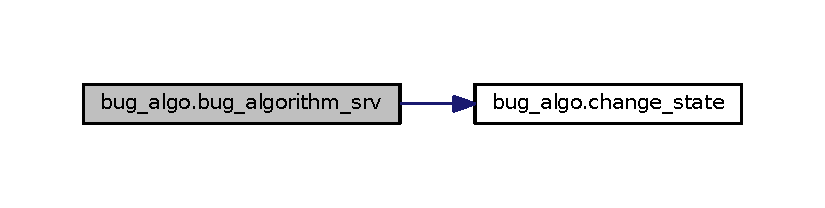
\includegraphics[width=350pt]{namespacebug__algo_afe2965502b3ec1efdb6ac2dadfb9a5de_cgraph}
\end{center}
\end{figure}


\index{bug\+\_\+algo@{bug\+\_\+algo}!change\+\_\+state@{change\+\_\+state}}
\index{change\+\_\+state@{change\+\_\+state}!bug\+\_\+algo@{bug\+\_\+algo}}
\subsubsection[{\texorpdfstring{change\+\_\+state(state)}{change_state(state)}}]{\setlength{\rightskip}{0pt plus 5cm}def bug\+\_\+algo.\+change\+\_\+state (
\begin{DoxyParamCaption}
\item[{}]{state}
\end{DoxyParamCaption}
)}\hypertarget{namespacebug__algo_aca287deda75aa8d0f790135ef47b6a16}{}\label{namespacebug__algo_aca287deda75aa8d0f790135ef47b6a16}


Change state function. 

manage the change of status of the robot, activating the corresponding services 
\begin{DoxyParams}{Parameters}
{\em state} & is the desired state \\
\hline
\end{DoxyParams}


Here is the caller graph for this function\+:\nopagebreak
\begin{figure}[H]
\begin{center}
\leavevmode
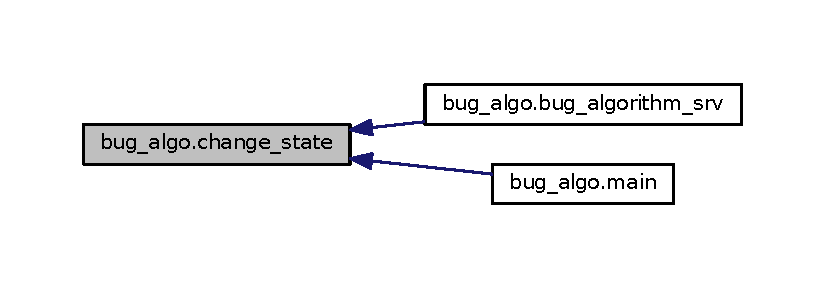
\includegraphics[width=350pt]{namespacebug__algo_aca287deda75aa8d0f790135ef47b6a16_icgraph}
\end{center}
\end{figure}


\index{bug\+\_\+algo@{bug\+\_\+algo}!clbk\+\_\+laser@{clbk\+\_\+laser}}
\index{clbk\+\_\+laser@{clbk\+\_\+laser}!bug\+\_\+algo@{bug\+\_\+algo}}
\subsubsection[{\texorpdfstring{clbk\+\_\+laser(msg)}{clbk_laser(msg)}}]{\setlength{\rightskip}{0pt plus 5cm}def bug\+\_\+algo.\+clbk\+\_\+laser (
\begin{DoxyParamCaption}
\item[{}]{msg}
\end{DoxyParamCaption}
)}\hypertarget{namespacebug__algo_a4363ca4faa041280e958c5141bc3bde8}{}\label{namespacebug__algo_a4363ca4faa041280e958c5141bc3bde8}


Laser data callback. 

output are localized in the robot in 5 regions organized as at the bottom variable regions\+\_\+ separes the output of lasers \index{bug\+\_\+algo@{bug\+\_\+algo}!clbk\+\_\+odom@{clbk\+\_\+odom}}
\index{clbk\+\_\+odom@{clbk\+\_\+odom}!bug\+\_\+algo@{bug\+\_\+algo}}
\subsubsection[{\texorpdfstring{clbk\+\_\+odom(msg)}{clbk_odom(msg)}}]{\setlength{\rightskip}{0pt plus 5cm}def bug\+\_\+algo.\+clbk\+\_\+odom (
\begin{DoxyParamCaption}
\item[{}]{msg}
\end{DoxyParamCaption}
)}\hypertarget{namespacebug__algo_a6a72a118f8a289bf80b1fe79487b273f}{}\label{namespacebug__algo_a6a72a118f8a289bf80b1fe79487b273f}


Function to retrieve robot pose. 

it\textquotesingle{}s the callback for the subscriber on topic /odom \index{bug\+\_\+algo@{bug\+\_\+algo}!main@{main}}
\index{main@{main}!bug\+\_\+algo@{bug\+\_\+algo}}
\subsubsection[{\texorpdfstring{main()}{main()}}]{\setlength{\rightskip}{0pt plus 5cm}def bug\+\_\+algo.\+main (
\begin{DoxyParamCaption}
{}
\end{DoxyParamCaption}
)}\hypertarget{namespacebug__algo_a8df2ef2049aa935d5478597523b50dcb}{}\label{namespacebug__algo_a8df2ef2049aa935d5478597523b50dcb}


Main function. 

Initalizes all the necessary pubs, subs ,clients and server It basically works as state machine with in addition some controls about the elapsed time that might result in aborting the reaching 

Here is the call graph for this function\+:\nopagebreak
\begin{figure}[H]
\begin{center}
\leavevmode
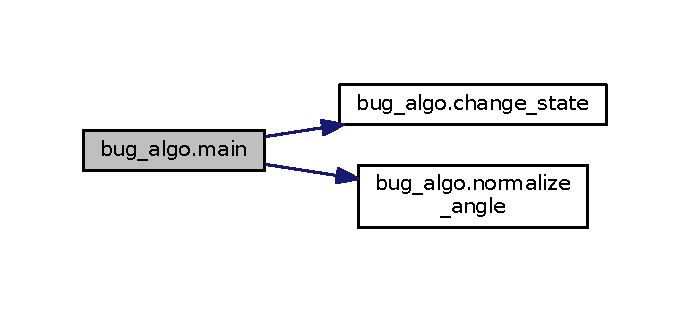
\includegraphics[width=331pt]{namespacebug__algo_a8df2ef2049aa935d5478597523b50dcb_cgraph}
\end{center}
\end{figure}


\index{bug\+\_\+algo@{bug\+\_\+algo}!normalize\+\_\+angle@{normalize\+\_\+angle}}
\index{normalize\+\_\+angle@{normalize\+\_\+angle}!bug\+\_\+algo@{bug\+\_\+algo}}
\subsubsection[{\texorpdfstring{normalize\+\_\+angle(angle)}{normalize_angle(angle)}}]{\setlength{\rightskip}{0pt plus 5cm}def bug\+\_\+algo.\+normalize\+\_\+angle (
\begin{DoxyParamCaption}
\item[{}]{angle}
\end{DoxyParamCaption}
)}\hypertarget{namespacebug__algo_ae499da57d8d88a30b64054480fdb60c8}{}\label{namespacebug__algo_ae499da57d8d88a30b64054480fdb60c8}


Normalize angle function. 

normalizes an angle 

Here is the caller graph for this function\+:\nopagebreak
\begin{figure}[H]
\begin{center}
\leavevmode
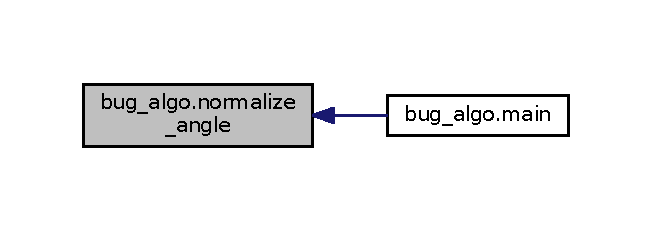
\includegraphics[width=313pt]{namespacebug__algo_ae499da57d8d88a30b64054480fdb60c8_icgraph}
\end{center}
\end{figure}




\subsection{Variable Documentation}
\index{bug\+\_\+algo@{bug\+\_\+algo}!active\+\_\+@{active\+\_\+}}
\index{active\+\_\+@{active\+\_\+}!bug\+\_\+algo@{bug\+\_\+algo}}
\subsubsection[{\texorpdfstring{active\+\_\+}{active_}}]{\setlength{\rightskip}{0pt plus 5cm}bool bug\+\_\+algo.\+active\+\_\+ = False}\hypertarget{namespacebug__algo_a3bec537d2bfc115b0a14ee6bad41bd00}{}\label{namespacebug__algo_a3bec537d2bfc115b0a14ee6bad41bd00}
\index{bug\+\_\+algo@{bug\+\_\+algo}!actual\+\_\+time@{actual\+\_\+time}}
\index{actual\+\_\+time@{actual\+\_\+time}!bug\+\_\+algo@{bug\+\_\+algo}}
\subsubsection[{\texorpdfstring{actual\+\_\+time}{actual_time}}]{\setlength{\rightskip}{0pt plus 5cm}int bug\+\_\+algo.\+actual\+\_\+time = 0}\hypertarget{namespacebug__algo_af9e77fe7842316d1491ef585c7602710}{}\label{namespacebug__algo_af9e77fe7842316d1491ef585c7602710}
\index{bug\+\_\+algo@{bug\+\_\+algo}!desired\+\_\+position\+\_\+@{desired\+\_\+position\+\_\+}}
\index{desired\+\_\+position\+\_\+@{desired\+\_\+position\+\_\+}!bug\+\_\+algo@{bug\+\_\+algo}}
\subsubsection[{\texorpdfstring{desired\+\_\+position\+\_\+}{desired_position_}}]{\setlength{\rightskip}{0pt plus 5cm}bug\+\_\+algo.\+desired\+\_\+position\+\_\+ = Point()}\hypertarget{namespacebug__algo_a6bc76d9dd5213819c8287c8833f8f3bd}{}\label{namespacebug__algo_a6bc76d9dd5213819c8287c8833f8f3bd}
\index{bug\+\_\+algo@{bug\+\_\+algo}!elapsed\+\_\+time@{elapsed\+\_\+time}}
\index{elapsed\+\_\+time@{elapsed\+\_\+time}!bug\+\_\+algo@{bug\+\_\+algo}}
\subsubsection[{\texorpdfstring{elapsed\+\_\+time}{elapsed_time}}]{\setlength{\rightskip}{0pt plus 5cm}int bug\+\_\+algo.\+elapsed\+\_\+time = 0}\hypertarget{namespacebug__algo_af723ba0d909555b34934483c74e06818}{}\label{namespacebug__algo_af723ba0d909555b34934483c74e06818}
\index{bug\+\_\+algo@{bug\+\_\+algo}!position\+\_\+@{position\+\_\+}}
\index{position\+\_\+@{position\+\_\+}!bug\+\_\+algo@{bug\+\_\+algo}}
\subsubsection[{\texorpdfstring{position\+\_\+}{position_}}]{\setlength{\rightskip}{0pt plus 5cm}bug\+\_\+algo.\+position\+\_\+ = Point()}\hypertarget{namespacebug__algo_ac0035ad008802f966f437b4787365220}{}\label{namespacebug__algo_ac0035ad008802f966f437b4787365220}
\index{bug\+\_\+algo@{bug\+\_\+algo}!pub@{pub}}
\index{pub@{pub}!bug\+\_\+algo@{bug\+\_\+algo}}
\subsubsection[{\texorpdfstring{pub}{pub}}]{\setlength{\rightskip}{0pt plus 5cm}bug\+\_\+algo.\+pub = None}\hypertarget{namespacebug__algo_a17a7504f2f0f6714f6ac31a43107fc31}{}\label{namespacebug__algo_a17a7504f2f0f6714f6ac31a43107fc31}
\index{bug\+\_\+algo@{bug\+\_\+algo}!regions\+\_\+@{regions\+\_\+}}
\index{regions\+\_\+@{regions\+\_\+}!bug\+\_\+algo@{bug\+\_\+algo}}
\subsubsection[{\texorpdfstring{regions\+\_\+}{regions_}}]{\setlength{\rightskip}{0pt plus 5cm}bug\+\_\+algo.\+regions\+\_\+ = None}\hypertarget{namespacebug__algo_a31fd6300649f8a600eb87ebed00b174f}{}\label{namespacebug__algo_a31fd6300649f8a600eb87ebed00b174f}
\index{bug\+\_\+algo@{bug\+\_\+algo}!srv\+\_\+client\+\_\+go\+\_\+to\+\_\+point\+\_\+@{srv\+\_\+client\+\_\+go\+\_\+to\+\_\+point\+\_\+}}
\index{srv\+\_\+client\+\_\+go\+\_\+to\+\_\+point\+\_\+@{srv\+\_\+client\+\_\+go\+\_\+to\+\_\+point\+\_\+}!bug\+\_\+algo@{bug\+\_\+algo}}
\subsubsection[{\texorpdfstring{srv\+\_\+client\+\_\+go\+\_\+to\+\_\+point\+\_\+}{srv_client_go_to_point_}}]{\setlength{\rightskip}{0pt plus 5cm}bug\+\_\+algo.\+srv\+\_\+client\+\_\+go\+\_\+to\+\_\+point\+\_\+ = None}\hypertarget{namespacebug__algo_a52e8d210b667d955534f12f59f191eb3}{}\label{namespacebug__algo_a52e8d210b667d955534f12f59f191eb3}
\index{bug\+\_\+algo@{bug\+\_\+algo}!srv\+\_\+client\+\_\+user\+\_\+interface\+\_\+@{srv\+\_\+client\+\_\+user\+\_\+interface\+\_\+}}
\index{srv\+\_\+client\+\_\+user\+\_\+interface\+\_\+@{srv\+\_\+client\+\_\+user\+\_\+interface\+\_\+}!bug\+\_\+algo@{bug\+\_\+algo}}
\subsubsection[{\texorpdfstring{srv\+\_\+client\+\_\+user\+\_\+interface\+\_\+}{srv_client_user_interface_}}]{\setlength{\rightskip}{0pt plus 5cm}bug\+\_\+algo.\+srv\+\_\+client\+\_\+user\+\_\+interface\+\_\+ = None}\hypertarget{namespacebug__algo_a1a55011236874d9af4afcf4c3524bbf0}{}\label{namespacebug__algo_a1a55011236874d9af4afcf4c3524bbf0}
\index{bug\+\_\+algo@{bug\+\_\+algo}!srv\+\_\+client\+\_\+user\+\_\+interface\+\_\+assignment\+\_\+@{srv\+\_\+client\+\_\+user\+\_\+interface\+\_\+assignment\+\_\+}}
\index{srv\+\_\+client\+\_\+user\+\_\+interface\+\_\+assignment\+\_\+@{srv\+\_\+client\+\_\+user\+\_\+interface\+\_\+assignment\+\_\+}!bug\+\_\+algo@{bug\+\_\+algo}}
\subsubsection[{\texorpdfstring{srv\+\_\+client\+\_\+user\+\_\+interface\+\_\+assignment\+\_\+}{srv_client_user_interface_assignment_}}]{\setlength{\rightskip}{0pt plus 5cm}bug\+\_\+algo.\+srv\+\_\+client\+\_\+user\+\_\+interface\+\_\+assignment\+\_\+ = None}\hypertarget{namespacebug__algo_ac9de3b470960260c4510748850446480}{}\label{namespacebug__algo_ac9de3b470960260c4510748850446480}
\index{bug\+\_\+algo@{bug\+\_\+algo}!srv\+\_\+client\+\_\+wall\+\_\+follower\+\_\+@{srv\+\_\+client\+\_\+wall\+\_\+follower\+\_\+}}
\index{srv\+\_\+client\+\_\+wall\+\_\+follower\+\_\+@{srv\+\_\+client\+\_\+wall\+\_\+follower\+\_\+}!bug\+\_\+algo@{bug\+\_\+algo}}
\subsubsection[{\texorpdfstring{srv\+\_\+client\+\_\+wall\+\_\+follower\+\_\+}{srv_client_wall_follower_}}]{\setlength{\rightskip}{0pt plus 5cm}bug\+\_\+algo.\+srv\+\_\+client\+\_\+wall\+\_\+follower\+\_\+ = None}\hypertarget{namespacebug__algo_afe0f6c6a1a9bc751e4bbcae499815585}{}\label{namespacebug__algo_afe0f6c6a1a9bc751e4bbcae499815585}
\index{bug\+\_\+algo@{bug\+\_\+algo}!start\+\_\+time@{start\+\_\+time}}
\index{start\+\_\+time@{start\+\_\+time}!bug\+\_\+algo@{bug\+\_\+algo}}
\subsubsection[{\texorpdfstring{start\+\_\+time}{start_time}}]{\setlength{\rightskip}{0pt plus 5cm}int bug\+\_\+algo.\+start\+\_\+time = 0}\hypertarget{namespacebug__algo_a6ff626c7bf6a4dfec4e8508d8ae5097c}{}\label{namespacebug__algo_a6ff626c7bf6a4dfec4e8508d8ae5097c}
\index{bug\+\_\+algo@{bug\+\_\+algo}!state\+\_\+@{state\+\_\+}}
\index{state\+\_\+@{state\+\_\+}!bug\+\_\+algo@{bug\+\_\+algo}}
\subsubsection[{\texorpdfstring{state\+\_\+}{state_}}]{\setlength{\rightskip}{0pt plus 5cm}int bug\+\_\+algo.\+state\+\_\+ = 0}\hypertarget{namespacebug__algo_a5bf52a66b7821a097f6e653a2422748e}{}\label{namespacebug__algo_a5bf52a66b7821a097f6e653a2422748e}
\index{bug\+\_\+algo@{bug\+\_\+algo}!state\+\_\+desc\+\_\+@{state\+\_\+desc\+\_\+}}
\index{state\+\_\+desc\+\_\+@{state\+\_\+desc\+\_\+}!bug\+\_\+algo@{bug\+\_\+algo}}
\subsubsection[{\texorpdfstring{state\+\_\+desc\+\_\+}{state_desc_}}]{\setlength{\rightskip}{0pt plus 5cm}list bug\+\_\+algo.\+state\+\_\+desc\+\_\+ = \mbox{[}\textquotesingle{}Go to point\textquotesingle{}, \textquotesingle{}wall following\textquotesingle{}, \textquotesingle{}stopped\textquotesingle{}\mbox{]}}\hypertarget{namespacebug__algo_a419cb7998b9a3946692fc01f5d73a25b}{}\label{namespacebug__algo_a419cb7998b9a3946692fc01f5d73a25b}
\index{bug\+\_\+algo@{bug\+\_\+algo}!x@{x}}
\index{x@{x}!bug\+\_\+algo@{bug\+\_\+algo}}
\subsubsection[{\texorpdfstring{x}{x}}]{\setlength{\rightskip}{0pt plus 5cm}bug\+\_\+algo.\+x}\hypertarget{namespacebug__algo_ae006850add8691db5d752b4ccb732ac1}{}\label{namespacebug__algo_ae006850add8691db5d752b4ccb732ac1}
\index{bug\+\_\+algo@{bug\+\_\+algo}!y@{y}}
\index{y@{y}!bug\+\_\+algo@{bug\+\_\+algo}}
\subsubsection[{\texorpdfstring{y}{y}}]{\setlength{\rightskip}{0pt plus 5cm}bug\+\_\+algo.\+y}\hypertarget{namespacebug__algo_a1e2d049a4b898c92454f0fb146a413ee}{}\label{namespacebug__algo_a1e2d049a4b898c92454f0fb146a413ee}
\index{bug\+\_\+algo@{bug\+\_\+algo}!yaw\+\_\+@{yaw\+\_\+}}
\index{yaw\+\_\+@{yaw\+\_\+}!bug\+\_\+algo@{bug\+\_\+algo}}
\subsubsection[{\texorpdfstring{yaw\+\_\+}{yaw_}}]{\setlength{\rightskip}{0pt plus 5cm}int bug\+\_\+algo.\+yaw\+\_\+ = 0}\hypertarget{namespacebug__algo_a2c8d86dd369e86415dc7ff9c617033d7}{}\label{namespacebug__algo_a2c8d86dd369e86415dc7ff9c617033d7}
\index{bug\+\_\+algo@{bug\+\_\+algo}!yaw\+\_\+error\+\_\+allowed\+\_\+@{yaw\+\_\+error\+\_\+allowed\+\_\+}}
\index{yaw\+\_\+error\+\_\+allowed\+\_\+@{yaw\+\_\+error\+\_\+allowed\+\_\+}!bug\+\_\+algo@{bug\+\_\+algo}}
\subsubsection[{\texorpdfstring{yaw\+\_\+error\+\_\+allowed\+\_\+}{yaw_error_allowed_}}]{\setlength{\rightskip}{0pt plus 5cm}int bug\+\_\+algo.\+yaw\+\_\+error\+\_\+allowed\+\_\+ = 5}\hypertarget{namespacebug__algo_a3714c955ff3cf688c84d6dc5654833d6}{}\label{namespacebug__algo_a3714c955ff3cf688c84d6dc5654833d6}
\index{bug\+\_\+algo@{bug\+\_\+algo}!z@{z}}
\index{z@{z}!bug\+\_\+algo@{bug\+\_\+algo}}
\subsubsection[{\texorpdfstring{z}{z}}]{\setlength{\rightskip}{0pt plus 5cm}bug\+\_\+algo.\+z}\hypertarget{namespacebug__algo_ad9944dcf5037184fbfbe3162935d2a57}{}\label{namespacebug__algo_ad9944dcf5037184fbfbe3162935d2a57}

\hypertarget{namespacefinal__assignment}{}\section{final\+\_\+assignment Namespace Reference}
\label{namespacefinal__assignment}\index{final\+\_\+assignment@{final\+\_\+assignment}}


This node is in charge of monitoring the state of the robot, and activate the corresping services and behaviour.  




\subsection{Detailed Description}
This node is in charge of monitoring the state of the robot, and activate the corresping services and behaviour. 

This node is used from bug algoritmh for behaviour wall follow.

This node implements the wall follower algoritm for navigation.

This node implements the user interface used by the bug algoritm.

This node implements the go to point behaviour for the bug algoritm.

This node implements the bug algoritm for navigation.

This node implements the main user interface.

As already said this node activates the corresponding services via the function change\+\_\+state(state), and for the first two behaviours it sets the new goal position with the function \hyperlink{namespacebig__brain_a4f091a106e4ba678afd9bc2df4f2789b}{new\+\_\+goal()}.

It\textquotesingle{}s used to manage the output on shell when the bug algoritm is N\+OT active

It\textquotesingle{}s used to manage the output on shell when the bug algoritm is activated

It works specifically when the bug algoritm is active

It works specifically when the bug algoritm is N\+OT active

the code is the same of \hyperlink{wall__follower__service_8py}{wall\+\_\+follower\+\_\+service.\+py} the comment are the same 
\hypertarget{namespacego__to__point__service__bug}{}\section{go\+\_\+to\+\_\+point\+\_\+service\+\_\+bug Namespace Reference}
\label{namespacego__to__point__service__bug}\index{go\+\_\+to\+\_\+point\+\_\+service\+\_\+bug@{go\+\_\+to\+\_\+point\+\_\+service\+\_\+bug}}
\subsection*{Functions}
\begin{DoxyCompactItemize}
\item 
def \hyperlink{namespacego__to__point__service__bug_a66835918820d392cf39cc1e3b28497ee}{go\+\_\+to\+\_\+point\+\_\+switch} (req)
\begin{DoxyCompactList}\small\item\em Function activated on service request. \end{DoxyCompactList}\item 
def \hyperlink{namespacego__to__point__service__bug_acc2367a3fc6946e8ea518d82a018dcd7}{clbk\+\_\+odom} (msg)
\begin{DoxyCompactList}\small\item\em Function to retrieve robot pose. \end{DoxyCompactList}\item 
def \hyperlink{namespacego__to__point__service__bug_a99587ca3714f1c59523a0fccdb4acc7d}{change\+\_\+state} (state)
\begin{DoxyCompactList}\small\item\em Change state function. \end{DoxyCompactList}\item 
def \hyperlink{namespacego__to__point__service__bug_a3ff83aec5e0de49fa33f2d33681d2a49}{normalize\+\_\+angle} (angle)
\begin{DoxyCompactList}\small\item\em Normalize angle function. \end{DoxyCompactList}\item 
def \hyperlink{namespacego__to__point__service__bug_a0f4f965c49e3e20c6442b10bf41e2533}{fix\+\_\+yaw} (des\+\_\+pos)
\begin{DoxyCompactList}\small\item\em Fix Yah function. \end{DoxyCompactList}\item 
def \hyperlink{namespacego__to__point__service__bug_a78a4659fd178f90a4b0acb3a4da0fbc1}{go\+\_\+straight\+\_\+ahead} (des\+\_\+pos)
\begin{DoxyCompactList}\small\item\em Go straight function. \end{DoxyCompactList}\item 
def \hyperlink{namespacego__to__point__service__bug_a181271bc83dc620614c43e6bd6b18db8}{done} (des\+\_\+pos)
\begin{DoxyCompactList}\small\item\em Done function. \end{DoxyCompactList}\item 
def \hyperlink{namespacego__to__point__service__bug_abb5a5a69905cef8ab5baf0768056ecea}{main} ()
\begin{DoxyCompactList}\small\item\em Main function. \end{DoxyCompactList}\end{DoxyCompactItemize}
\subsection*{Variables}
\begin{DoxyCompactItemize}
\item 
bool \hyperlink{namespacego__to__point__service__bug_a904337d36bd7e3e63dc3d862b0f67608}{active\+\_\+} = False
\item 
\hyperlink{namespacego__to__point__service__bug_a8eccd57782f5a63758c2ed6fc429648f}{position\+\_\+} = Point()
\item 
int \hyperlink{namespacego__to__point__service__bug_a92ae1b18b13762d59aa27dd83ea9e04d}{yaw\+\_\+} = 0
\item 
int \hyperlink{namespacego__to__point__service__bug_acf82697453e220209d6f386e1630619a}{state\+\_\+} = 0
\item 
\hyperlink{namespacego__to__point__service__bug_a5c33b74b7f2376e73690f8474fc4db36}{desired\+\_\+position\+\_\+} = Point()
\item 
\hyperlink{namespacego__to__point__service__bug_a6761dc57b29d40d3e6578b775a1e84c2}{x}
\item 
\hyperlink{namespacego__to__point__service__bug_a9eac097a440f4f16c9e7260e5296fd76}{y}
\item 
\hyperlink{namespacego__to__point__service__bug_ac72a9ad64f48ea907c94e25a3718372c}{z}
\item 
int \hyperlink{namespacego__to__point__service__bug_aa27745ad563c25adbac628695bbdd44d}{yaw\+\_\+precision\+\_\+} = math.\+pi/9
\item 
int \hyperlink{namespacego__to__point__service__bug_a2cfb8eb9d839627bee23494c162a1e88}{yaw\+\_\+precision\+\_\+2\+\_\+} = math.\+pi/90
\item 
float \hyperlink{namespacego__to__point__service__bug_a1142014aa3b5c0819cd183c7b4534927}{dist\+\_\+precision\+\_\+} = 0.\+3
\item 
float \hyperlink{namespacego__to__point__service__bug_ab4d1411316c963d5b211e42f78cf3c93}{kp\+\_\+a} = 3.\+0
\item 
float \hyperlink{namespacego__to__point__service__bug_a0aa73d2814be9d22fc2a6e4eaa0afc07}{kp\+\_\+d} = 0.\+2
\item 
float \hyperlink{namespacego__to__point__service__bug_aa2cfb37c171e32902af10e4f4121f92f}{ub\+\_\+a} = 0.\+6
\item 
float \hyperlink{namespacego__to__point__service__bug_a60404a026e5fcd840f8a6f712edfb71f}{lb\+\_\+a} = -\/0.\+5
\item 
float \hyperlink{namespacego__to__point__service__bug_a0ea364ac6b209e590e96109ca6fb7a5c}{ub\+\_\+d} = 0.\+6
\item 
\hyperlink{namespacego__to__point__service__bug_a303812c1ccf752e711d273e93c27293d}{pub} = None
\end{DoxyCompactItemize}


\subsection{Function Documentation}
\index{go\+\_\+to\+\_\+point\+\_\+service\+\_\+bug@{go\+\_\+to\+\_\+point\+\_\+service\+\_\+bug}!change\+\_\+state@{change\+\_\+state}}
\index{change\+\_\+state@{change\+\_\+state}!go\+\_\+to\+\_\+point\+\_\+service\+\_\+bug@{go\+\_\+to\+\_\+point\+\_\+service\+\_\+bug}}
\subsubsection[{\texorpdfstring{change\+\_\+state(state)}{change_state(state)}}]{\setlength{\rightskip}{0pt plus 5cm}def go\+\_\+to\+\_\+point\+\_\+service\+\_\+bug.\+change\+\_\+state (
\begin{DoxyParamCaption}
\item[{}]{state}
\end{DoxyParamCaption}
)}\hypertarget{namespacego__to__point__service__bug_a99587ca3714f1c59523a0fccdb4acc7d}{}\label{namespacego__to__point__service__bug_a99587ca3714f1c59523a0fccdb4acc7d}


Change state function. 

manage the change of status of the robot 

Here is the caller graph for this function\+:\nopagebreak
\begin{figure}[H]
\begin{center}
\leavevmode
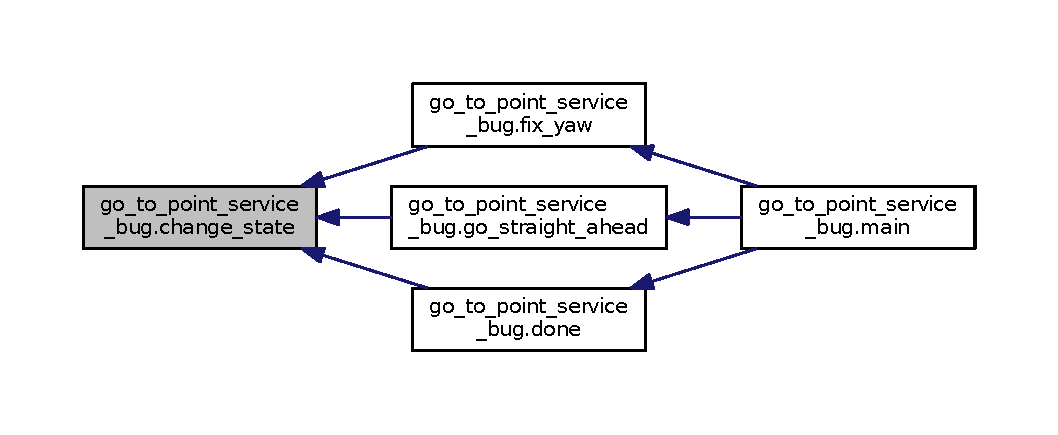
\includegraphics[width=350pt]{namespacego__to__point__service__bug_a99587ca3714f1c59523a0fccdb4acc7d_icgraph}
\end{center}
\end{figure}


\index{go\+\_\+to\+\_\+point\+\_\+service\+\_\+bug@{go\+\_\+to\+\_\+point\+\_\+service\+\_\+bug}!clbk\+\_\+odom@{clbk\+\_\+odom}}
\index{clbk\+\_\+odom@{clbk\+\_\+odom}!go\+\_\+to\+\_\+point\+\_\+service\+\_\+bug@{go\+\_\+to\+\_\+point\+\_\+service\+\_\+bug}}
\subsubsection[{\texorpdfstring{clbk\+\_\+odom(msg)}{clbk_odom(msg)}}]{\setlength{\rightskip}{0pt plus 5cm}def go\+\_\+to\+\_\+point\+\_\+service\+\_\+bug.\+clbk\+\_\+odom (
\begin{DoxyParamCaption}
\item[{}]{msg}
\end{DoxyParamCaption}
)}\hypertarget{namespacego__to__point__service__bug_acc2367a3fc6946e8ea518d82a018dcd7}{}\label{namespacego__to__point__service__bug_acc2367a3fc6946e8ea518d82a018dcd7}


Function to retrieve robot pose. 

it\textquotesingle{}s the callback for the subscriber on topic /odom \index{go\+\_\+to\+\_\+point\+\_\+service\+\_\+bug@{go\+\_\+to\+\_\+point\+\_\+service\+\_\+bug}!done@{done}}
\index{done@{done}!go\+\_\+to\+\_\+point\+\_\+service\+\_\+bug@{go\+\_\+to\+\_\+point\+\_\+service\+\_\+bug}}
\subsubsection[{\texorpdfstring{done(des\+\_\+pos)}{done(des_pos)}}]{\setlength{\rightskip}{0pt plus 5cm}def go\+\_\+to\+\_\+point\+\_\+service\+\_\+bug.\+done (
\begin{DoxyParamCaption}
\item[{}]{des\+\_\+pos}
\end{DoxyParamCaption}
)}\hypertarget{namespacego__to__point__service__bug_a181271bc83dc620614c43e6bd6b18db8}{}\label{namespacego__to__point__service__bug_a181271bc83dc620614c43e6bd6b18db8}


Done function. 

stops the robot once it has reached a goal 

Here is the call graph for this function\+:\nopagebreak
\begin{figure}[H]
\begin{center}
\leavevmode
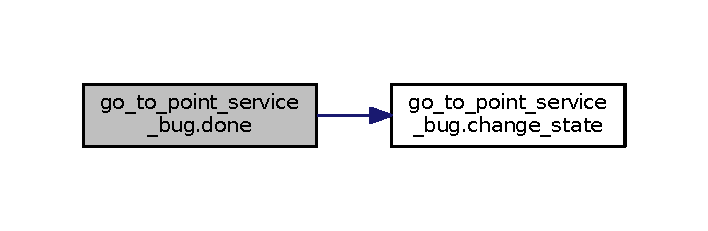
\includegraphics[width=340pt]{namespacego__to__point__service__bug_a181271bc83dc620614c43e6bd6b18db8_cgraph}
\end{center}
\end{figure}




Here is the caller graph for this function\+:\nopagebreak
\begin{figure}[H]
\begin{center}
\leavevmode
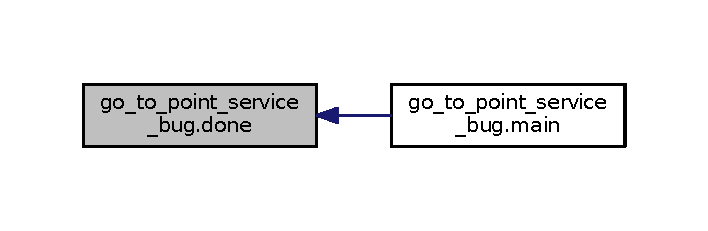
\includegraphics[width=340pt]{namespacego__to__point__service__bug_a181271bc83dc620614c43e6bd6b18db8_icgraph}
\end{center}
\end{figure}


\index{go\+\_\+to\+\_\+point\+\_\+service\+\_\+bug@{go\+\_\+to\+\_\+point\+\_\+service\+\_\+bug}!fix\+\_\+yaw@{fix\+\_\+yaw}}
\index{fix\+\_\+yaw@{fix\+\_\+yaw}!go\+\_\+to\+\_\+point\+\_\+service\+\_\+bug@{go\+\_\+to\+\_\+point\+\_\+service\+\_\+bug}}
\subsubsection[{\texorpdfstring{fix\+\_\+yaw(des\+\_\+pos)}{fix_yaw(des_pos)}}]{\setlength{\rightskip}{0pt plus 5cm}def go\+\_\+to\+\_\+point\+\_\+service\+\_\+bug.\+fix\+\_\+yaw (
\begin{DoxyParamCaption}
\item[{}]{des\+\_\+pos}
\end{DoxyParamCaption}
)}\hypertarget{namespacego__to__point__service__bug_a0f4f965c49e3e20c6442b10bf41e2533}{}\label{namespacego__to__point__service__bug_a0f4f965c49e3e20c6442b10bf41e2533}


Fix Yah function. 

fixes the orientation of the robot 

Here is the call graph for this function\+:\nopagebreak
\begin{figure}[H]
\begin{center}
\leavevmode
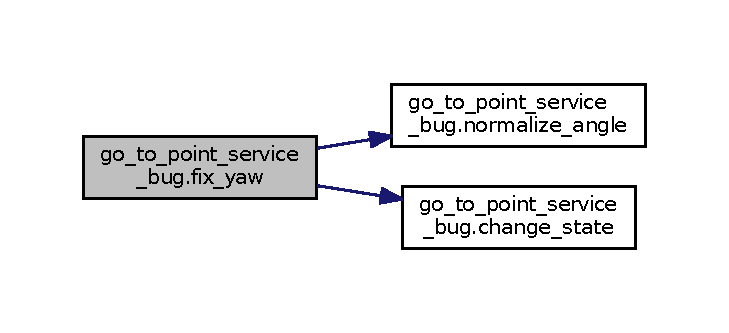
\includegraphics[width=350pt]{namespacego__to__point__service__bug_a0f4f965c49e3e20c6442b10bf41e2533_cgraph}
\end{center}
\end{figure}




Here is the caller graph for this function\+:\nopagebreak
\begin{figure}[H]
\begin{center}
\leavevmode
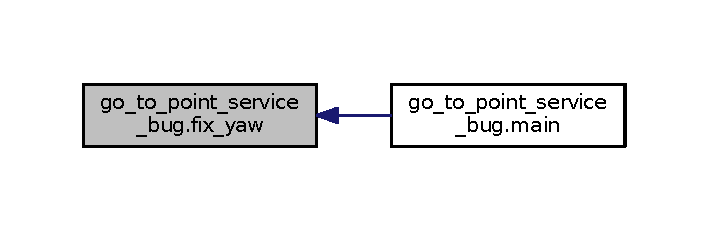
\includegraphics[width=340pt]{namespacego__to__point__service__bug_a0f4f965c49e3e20c6442b10bf41e2533_icgraph}
\end{center}
\end{figure}


\index{go\+\_\+to\+\_\+point\+\_\+service\+\_\+bug@{go\+\_\+to\+\_\+point\+\_\+service\+\_\+bug}!go\+\_\+straight\+\_\+ahead@{go\+\_\+straight\+\_\+ahead}}
\index{go\+\_\+straight\+\_\+ahead@{go\+\_\+straight\+\_\+ahead}!go\+\_\+to\+\_\+point\+\_\+service\+\_\+bug@{go\+\_\+to\+\_\+point\+\_\+service\+\_\+bug}}
\subsubsection[{\texorpdfstring{go\+\_\+straight\+\_\+ahead(des\+\_\+pos)}{go_straight_ahead(des_pos)}}]{\setlength{\rightskip}{0pt plus 5cm}def go\+\_\+to\+\_\+point\+\_\+service\+\_\+bug.\+go\+\_\+straight\+\_\+ahead (
\begin{DoxyParamCaption}
\item[{}]{des\+\_\+pos}
\end{DoxyParamCaption}
)}\hypertarget{namespacego__to__point__service__bug_a78a4659fd178f90a4b0acb3a4da0fbc1}{}\label{namespacego__to__point__service__bug_a78a4659fd178f90a4b0acb3a4da0fbc1}


Go straight function. 

publishes on cmd\+\_\+vel to make the robot go straight 

Here is the call graph for this function\+:\nopagebreak
\begin{figure}[H]
\begin{center}
\leavevmode
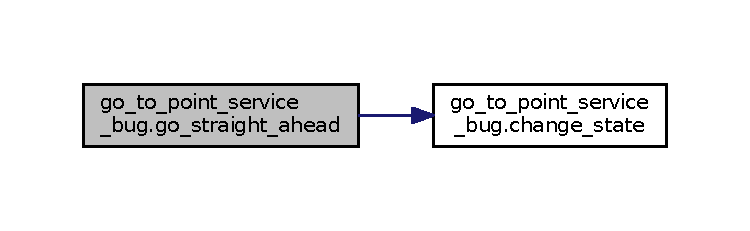
\includegraphics[width=350pt]{namespacego__to__point__service__bug_a78a4659fd178f90a4b0acb3a4da0fbc1_cgraph}
\end{center}
\end{figure}




Here is the caller graph for this function\+:\nopagebreak
\begin{figure}[H]
\begin{center}
\leavevmode
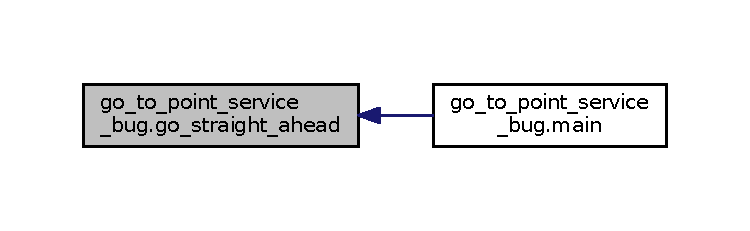
\includegraphics[width=350pt]{namespacego__to__point__service__bug_a78a4659fd178f90a4b0acb3a4da0fbc1_icgraph}
\end{center}
\end{figure}


\index{go\+\_\+to\+\_\+point\+\_\+service\+\_\+bug@{go\+\_\+to\+\_\+point\+\_\+service\+\_\+bug}!go\+\_\+to\+\_\+point\+\_\+switch@{go\+\_\+to\+\_\+point\+\_\+switch}}
\index{go\+\_\+to\+\_\+point\+\_\+switch@{go\+\_\+to\+\_\+point\+\_\+switch}!go\+\_\+to\+\_\+point\+\_\+service\+\_\+bug@{go\+\_\+to\+\_\+point\+\_\+service\+\_\+bug}}
\subsubsection[{\texorpdfstring{go\+\_\+to\+\_\+point\+\_\+switch(req)}{go_to_point_switch(req)}}]{\setlength{\rightskip}{0pt plus 5cm}def go\+\_\+to\+\_\+point\+\_\+service\+\_\+bug.\+go\+\_\+to\+\_\+point\+\_\+switch (
\begin{DoxyParamCaption}
\item[{}]{req}
\end{DoxyParamCaption}
)}\hypertarget{namespacego__to__point__service__bug_a66835918820d392cf39cc1e3b28497ee}{}\label{namespacego__to__point__service__bug_a66835918820d392cf39cc1e3b28497ee}


Function activated on service request. 


\begin{DoxyParams}{Parameters}
{\em req} & is the request of the service \\
\hline
\end{DoxyParams}
\index{go\+\_\+to\+\_\+point\+\_\+service\+\_\+bug@{go\+\_\+to\+\_\+point\+\_\+service\+\_\+bug}!main@{main}}
\index{main@{main}!go\+\_\+to\+\_\+point\+\_\+service\+\_\+bug@{go\+\_\+to\+\_\+point\+\_\+service\+\_\+bug}}
\subsubsection[{\texorpdfstring{main()}{main()}}]{\setlength{\rightskip}{0pt plus 5cm}def go\+\_\+to\+\_\+point\+\_\+service\+\_\+bug.\+main (
\begin{DoxyParamCaption}
{}
\end{DoxyParamCaption}
)}\hypertarget{namespacego__to__point__service__bug_abb5a5a69905cef8ab5baf0768056ecea}{}\label{namespacego__to__point__service__bug_abb5a5a69905cef8ab5baf0768056ecea}


Main function. 

initializes necessary variables, works as a state machine 

Here is the call graph for this function\+:\nopagebreak
\begin{figure}[H]
\begin{center}
\leavevmode
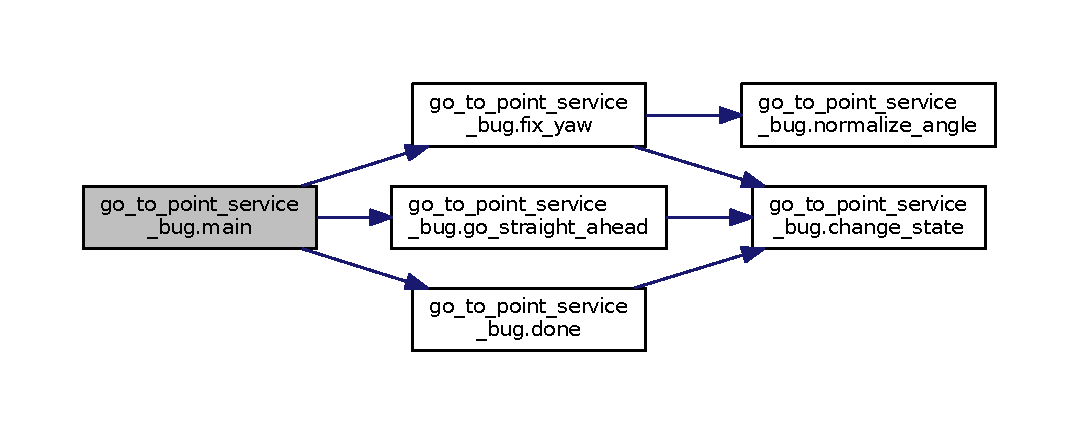
\includegraphics[width=350pt]{namespacego__to__point__service__bug_abb5a5a69905cef8ab5baf0768056ecea_cgraph}
\end{center}
\end{figure}


\index{go\+\_\+to\+\_\+point\+\_\+service\+\_\+bug@{go\+\_\+to\+\_\+point\+\_\+service\+\_\+bug}!normalize\+\_\+angle@{normalize\+\_\+angle}}
\index{normalize\+\_\+angle@{normalize\+\_\+angle}!go\+\_\+to\+\_\+point\+\_\+service\+\_\+bug@{go\+\_\+to\+\_\+point\+\_\+service\+\_\+bug}}
\subsubsection[{\texorpdfstring{normalize\+\_\+angle(angle)}{normalize_angle(angle)}}]{\setlength{\rightskip}{0pt plus 5cm}def go\+\_\+to\+\_\+point\+\_\+service\+\_\+bug.\+normalize\+\_\+angle (
\begin{DoxyParamCaption}
\item[{}]{angle}
\end{DoxyParamCaption}
)}\hypertarget{namespacego__to__point__service__bug_a3ff83aec5e0de49fa33f2d33681d2a49}{}\label{namespacego__to__point__service__bug_a3ff83aec5e0de49fa33f2d33681d2a49}


Normalize angle function. 

normalizes an angle 

Here is the caller graph for this function\+:\nopagebreak
\begin{figure}[H]
\begin{center}
\leavevmode
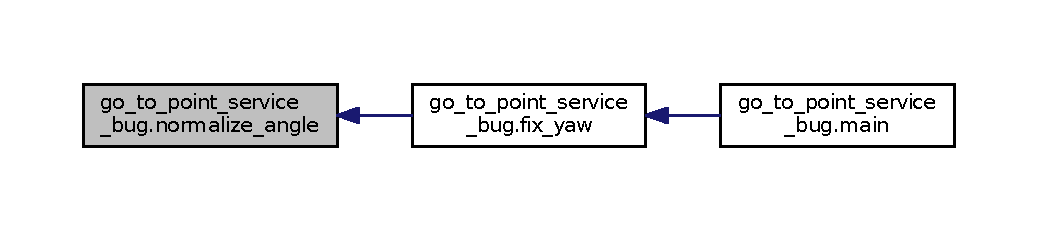
\includegraphics[width=350pt]{namespacego__to__point__service__bug_a3ff83aec5e0de49fa33f2d33681d2a49_icgraph}
\end{center}
\end{figure}




\subsection{Variable Documentation}
\index{go\+\_\+to\+\_\+point\+\_\+service\+\_\+bug@{go\+\_\+to\+\_\+point\+\_\+service\+\_\+bug}!active\+\_\+@{active\+\_\+}}
\index{active\+\_\+@{active\+\_\+}!go\+\_\+to\+\_\+point\+\_\+service\+\_\+bug@{go\+\_\+to\+\_\+point\+\_\+service\+\_\+bug}}
\subsubsection[{\texorpdfstring{active\+\_\+}{active_}}]{\setlength{\rightskip}{0pt plus 5cm}bool go\+\_\+to\+\_\+point\+\_\+service\+\_\+bug.\+active\+\_\+ = False}\hypertarget{namespacego__to__point__service__bug_a904337d36bd7e3e63dc3d862b0f67608}{}\label{namespacego__to__point__service__bug_a904337d36bd7e3e63dc3d862b0f67608}
\index{go\+\_\+to\+\_\+point\+\_\+service\+\_\+bug@{go\+\_\+to\+\_\+point\+\_\+service\+\_\+bug}!desired\+\_\+position\+\_\+@{desired\+\_\+position\+\_\+}}
\index{desired\+\_\+position\+\_\+@{desired\+\_\+position\+\_\+}!go\+\_\+to\+\_\+point\+\_\+service\+\_\+bug@{go\+\_\+to\+\_\+point\+\_\+service\+\_\+bug}}
\subsubsection[{\texorpdfstring{desired\+\_\+position\+\_\+}{desired_position_}}]{\setlength{\rightskip}{0pt plus 5cm}go\+\_\+to\+\_\+point\+\_\+service\+\_\+bug.\+desired\+\_\+position\+\_\+ = Point()}\hypertarget{namespacego__to__point__service__bug_a5c33b74b7f2376e73690f8474fc4db36}{}\label{namespacego__to__point__service__bug_a5c33b74b7f2376e73690f8474fc4db36}
\index{go\+\_\+to\+\_\+point\+\_\+service\+\_\+bug@{go\+\_\+to\+\_\+point\+\_\+service\+\_\+bug}!dist\+\_\+precision\+\_\+@{dist\+\_\+precision\+\_\+}}
\index{dist\+\_\+precision\+\_\+@{dist\+\_\+precision\+\_\+}!go\+\_\+to\+\_\+point\+\_\+service\+\_\+bug@{go\+\_\+to\+\_\+point\+\_\+service\+\_\+bug}}
\subsubsection[{\texorpdfstring{dist\+\_\+precision\+\_\+}{dist_precision_}}]{\setlength{\rightskip}{0pt plus 5cm}float go\+\_\+to\+\_\+point\+\_\+service\+\_\+bug.\+dist\+\_\+precision\+\_\+ = 0.\+3}\hypertarget{namespacego__to__point__service__bug_a1142014aa3b5c0819cd183c7b4534927}{}\label{namespacego__to__point__service__bug_a1142014aa3b5c0819cd183c7b4534927}
\index{go\+\_\+to\+\_\+point\+\_\+service\+\_\+bug@{go\+\_\+to\+\_\+point\+\_\+service\+\_\+bug}!kp\+\_\+a@{kp\+\_\+a}}
\index{kp\+\_\+a@{kp\+\_\+a}!go\+\_\+to\+\_\+point\+\_\+service\+\_\+bug@{go\+\_\+to\+\_\+point\+\_\+service\+\_\+bug}}
\subsubsection[{\texorpdfstring{kp\+\_\+a}{kp_a}}]{\setlength{\rightskip}{0pt plus 5cm}float go\+\_\+to\+\_\+point\+\_\+service\+\_\+bug.\+kp\+\_\+a = 3.\+0}\hypertarget{namespacego__to__point__service__bug_ab4d1411316c963d5b211e42f78cf3c93}{}\label{namespacego__to__point__service__bug_ab4d1411316c963d5b211e42f78cf3c93}
\index{go\+\_\+to\+\_\+point\+\_\+service\+\_\+bug@{go\+\_\+to\+\_\+point\+\_\+service\+\_\+bug}!kp\+\_\+d@{kp\+\_\+d}}
\index{kp\+\_\+d@{kp\+\_\+d}!go\+\_\+to\+\_\+point\+\_\+service\+\_\+bug@{go\+\_\+to\+\_\+point\+\_\+service\+\_\+bug}}
\subsubsection[{\texorpdfstring{kp\+\_\+d}{kp_d}}]{\setlength{\rightskip}{0pt plus 5cm}float go\+\_\+to\+\_\+point\+\_\+service\+\_\+bug.\+kp\+\_\+d = 0.\+2}\hypertarget{namespacego__to__point__service__bug_a0aa73d2814be9d22fc2a6e4eaa0afc07}{}\label{namespacego__to__point__service__bug_a0aa73d2814be9d22fc2a6e4eaa0afc07}
\index{go\+\_\+to\+\_\+point\+\_\+service\+\_\+bug@{go\+\_\+to\+\_\+point\+\_\+service\+\_\+bug}!lb\+\_\+a@{lb\+\_\+a}}
\index{lb\+\_\+a@{lb\+\_\+a}!go\+\_\+to\+\_\+point\+\_\+service\+\_\+bug@{go\+\_\+to\+\_\+point\+\_\+service\+\_\+bug}}
\subsubsection[{\texorpdfstring{lb\+\_\+a}{lb_a}}]{\setlength{\rightskip}{0pt plus 5cm}float go\+\_\+to\+\_\+point\+\_\+service\+\_\+bug.\+lb\+\_\+a = -\/0.\+5}\hypertarget{namespacego__to__point__service__bug_a60404a026e5fcd840f8a6f712edfb71f}{}\label{namespacego__to__point__service__bug_a60404a026e5fcd840f8a6f712edfb71f}
\index{go\+\_\+to\+\_\+point\+\_\+service\+\_\+bug@{go\+\_\+to\+\_\+point\+\_\+service\+\_\+bug}!position\+\_\+@{position\+\_\+}}
\index{position\+\_\+@{position\+\_\+}!go\+\_\+to\+\_\+point\+\_\+service\+\_\+bug@{go\+\_\+to\+\_\+point\+\_\+service\+\_\+bug}}
\subsubsection[{\texorpdfstring{position\+\_\+}{position_}}]{\setlength{\rightskip}{0pt plus 5cm}go\+\_\+to\+\_\+point\+\_\+service\+\_\+bug.\+position\+\_\+ = Point()}\hypertarget{namespacego__to__point__service__bug_a8eccd57782f5a63758c2ed6fc429648f}{}\label{namespacego__to__point__service__bug_a8eccd57782f5a63758c2ed6fc429648f}
\index{go\+\_\+to\+\_\+point\+\_\+service\+\_\+bug@{go\+\_\+to\+\_\+point\+\_\+service\+\_\+bug}!pub@{pub}}
\index{pub@{pub}!go\+\_\+to\+\_\+point\+\_\+service\+\_\+bug@{go\+\_\+to\+\_\+point\+\_\+service\+\_\+bug}}
\subsubsection[{\texorpdfstring{pub}{pub}}]{\setlength{\rightskip}{0pt plus 5cm}go\+\_\+to\+\_\+point\+\_\+service\+\_\+bug.\+pub = None}\hypertarget{namespacego__to__point__service__bug_a303812c1ccf752e711d273e93c27293d}{}\label{namespacego__to__point__service__bug_a303812c1ccf752e711d273e93c27293d}
\index{go\+\_\+to\+\_\+point\+\_\+service\+\_\+bug@{go\+\_\+to\+\_\+point\+\_\+service\+\_\+bug}!state\+\_\+@{state\+\_\+}}
\index{state\+\_\+@{state\+\_\+}!go\+\_\+to\+\_\+point\+\_\+service\+\_\+bug@{go\+\_\+to\+\_\+point\+\_\+service\+\_\+bug}}
\subsubsection[{\texorpdfstring{state\+\_\+}{state_}}]{\setlength{\rightskip}{0pt plus 5cm}int go\+\_\+to\+\_\+point\+\_\+service\+\_\+bug.\+state\+\_\+ = 0}\hypertarget{namespacego__to__point__service__bug_acf82697453e220209d6f386e1630619a}{}\label{namespacego__to__point__service__bug_acf82697453e220209d6f386e1630619a}
\index{go\+\_\+to\+\_\+point\+\_\+service\+\_\+bug@{go\+\_\+to\+\_\+point\+\_\+service\+\_\+bug}!ub\+\_\+a@{ub\+\_\+a}}
\index{ub\+\_\+a@{ub\+\_\+a}!go\+\_\+to\+\_\+point\+\_\+service\+\_\+bug@{go\+\_\+to\+\_\+point\+\_\+service\+\_\+bug}}
\subsubsection[{\texorpdfstring{ub\+\_\+a}{ub_a}}]{\setlength{\rightskip}{0pt plus 5cm}float go\+\_\+to\+\_\+point\+\_\+service\+\_\+bug.\+ub\+\_\+a = 0.\+6}\hypertarget{namespacego__to__point__service__bug_aa2cfb37c171e32902af10e4f4121f92f}{}\label{namespacego__to__point__service__bug_aa2cfb37c171e32902af10e4f4121f92f}
\index{go\+\_\+to\+\_\+point\+\_\+service\+\_\+bug@{go\+\_\+to\+\_\+point\+\_\+service\+\_\+bug}!ub\+\_\+d@{ub\+\_\+d}}
\index{ub\+\_\+d@{ub\+\_\+d}!go\+\_\+to\+\_\+point\+\_\+service\+\_\+bug@{go\+\_\+to\+\_\+point\+\_\+service\+\_\+bug}}
\subsubsection[{\texorpdfstring{ub\+\_\+d}{ub_d}}]{\setlength{\rightskip}{0pt plus 5cm}float go\+\_\+to\+\_\+point\+\_\+service\+\_\+bug.\+ub\+\_\+d = 0.\+6}\hypertarget{namespacego__to__point__service__bug_a0ea364ac6b209e590e96109ca6fb7a5c}{}\label{namespacego__to__point__service__bug_a0ea364ac6b209e590e96109ca6fb7a5c}
\index{go\+\_\+to\+\_\+point\+\_\+service\+\_\+bug@{go\+\_\+to\+\_\+point\+\_\+service\+\_\+bug}!x@{x}}
\index{x@{x}!go\+\_\+to\+\_\+point\+\_\+service\+\_\+bug@{go\+\_\+to\+\_\+point\+\_\+service\+\_\+bug}}
\subsubsection[{\texorpdfstring{x}{x}}]{\setlength{\rightskip}{0pt plus 5cm}go\+\_\+to\+\_\+point\+\_\+service\+\_\+bug.\+x}\hypertarget{namespacego__to__point__service__bug_a6761dc57b29d40d3e6578b775a1e84c2}{}\label{namespacego__to__point__service__bug_a6761dc57b29d40d3e6578b775a1e84c2}
\index{go\+\_\+to\+\_\+point\+\_\+service\+\_\+bug@{go\+\_\+to\+\_\+point\+\_\+service\+\_\+bug}!y@{y}}
\index{y@{y}!go\+\_\+to\+\_\+point\+\_\+service\+\_\+bug@{go\+\_\+to\+\_\+point\+\_\+service\+\_\+bug}}
\subsubsection[{\texorpdfstring{y}{y}}]{\setlength{\rightskip}{0pt plus 5cm}go\+\_\+to\+\_\+point\+\_\+service\+\_\+bug.\+y}\hypertarget{namespacego__to__point__service__bug_a9eac097a440f4f16c9e7260e5296fd76}{}\label{namespacego__to__point__service__bug_a9eac097a440f4f16c9e7260e5296fd76}
\index{go\+\_\+to\+\_\+point\+\_\+service\+\_\+bug@{go\+\_\+to\+\_\+point\+\_\+service\+\_\+bug}!yaw\+\_\+@{yaw\+\_\+}}
\index{yaw\+\_\+@{yaw\+\_\+}!go\+\_\+to\+\_\+point\+\_\+service\+\_\+bug@{go\+\_\+to\+\_\+point\+\_\+service\+\_\+bug}}
\subsubsection[{\texorpdfstring{yaw\+\_\+}{yaw_}}]{\setlength{\rightskip}{0pt plus 5cm}int go\+\_\+to\+\_\+point\+\_\+service\+\_\+bug.\+yaw\+\_\+ = 0}\hypertarget{namespacego__to__point__service__bug_a92ae1b18b13762d59aa27dd83ea9e04d}{}\label{namespacego__to__point__service__bug_a92ae1b18b13762d59aa27dd83ea9e04d}
\index{go\+\_\+to\+\_\+point\+\_\+service\+\_\+bug@{go\+\_\+to\+\_\+point\+\_\+service\+\_\+bug}!yaw\+\_\+precision\+\_\+@{yaw\+\_\+precision\+\_\+}}
\index{yaw\+\_\+precision\+\_\+@{yaw\+\_\+precision\+\_\+}!go\+\_\+to\+\_\+point\+\_\+service\+\_\+bug@{go\+\_\+to\+\_\+point\+\_\+service\+\_\+bug}}
\subsubsection[{\texorpdfstring{yaw\+\_\+precision\+\_\+}{yaw_precision_}}]{\setlength{\rightskip}{0pt plus 5cm}int go\+\_\+to\+\_\+point\+\_\+service\+\_\+bug.\+yaw\+\_\+precision\+\_\+ = math.\+pi/9}\hypertarget{namespacego__to__point__service__bug_aa27745ad563c25adbac628695bbdd44d}{}\label{namespacego__to__point__service__bug_aa27745ad563c25adbac628695bbdd44d}
\index{go\+\_\+to\+\_\+point\+\_\+service\+\_\+bug@{go\+\_\+to\+\_\+point\+\_\+service\+\_\+bug}!yaw\+\_\+precision\+\_\+2\+\_\+@{yaw\+\_\+precision\+\_\+2\+\_\+}}
\index{yaw\+\_\+precision\+\_\+2\+\_\+@{yaw\+\_\+precision\+\_\+2\+\_\+}!go\+\_\+to\+\_\+point\+\_\+service\+\_\+bug@{go\+\_\+to\+\_\+point\+\_\+service\+\_\+bug}}
\subsubsection[{\texorpdfstring{yaw\+\_\+precision\+\_\+2\+\_\+}{yaw_precision_2_}}]{\setlength{\rightskip}{0pt plus 5cm}int go\+\_\+to\+\_\+point\+\_\+service\+\_\+bug.\+yaw\+\_\+precision\+\_\+2\+\_\+ = math.\+pi/90}\hypertarget{namespacego__to__point__service__bug_a2cfb8eb9d839627bee23494c162a1e88}{}\label{namespacego__to__point__service__bug_a2cfb8eb9d839627bee23494c162a1e88}
\index{go\+\_\+to\+\_\+point\+\_\+service\+\_\+bug@{go\+\_\+to\+\_\+point\+\_\+service\+\_\+bug}!z@{z}}
\index{z@{z}!go\+\_\+to\+\_\+point\+\_\+service\+\_\+bug@{go\+\_\+to\+\_\+point\+\_\+service\+\_\+bug}}
\subsubsection[{\texorpdfstring{z}{z}}]{\setlength{\rightskip}{0pt plus 5cm}go\+\_\+to\+\_\+point\+\_\+service\+\_\+bug.\+z}\hypertarget{namespacego__to__point__service__bug_ac72a9ad64f48ea907c94e25a3718372c}{}\label{namespacego__to__point__service__bug_ac72a9ad64f48ea907c94e25a3718372c}

\hypertarget{namespaceuser__interface}{}\section{user\+\_\+interface Namespace Reference}
\label{namespaceuser__interface}\index{user\+\_\+interface@{user\+\_\+interface}}
\subsection*{Functions}
\begin{DoxyCompactItemize}
\item 
def \hyperlink{namespaceuser__interface_aa9dc3b0346ac037400ae347eb6efb788}{set\+\_\+new\+\_\+pos} (req)
\begin{DoxyCompactList}\small\item\em Function to set the new position for bug algoritm. \end{DoxyCompactList}\item 
def \hyperlink{namespaceuser__interface_ac26bdb296b6776907b72c17ce5a1b24a}{main} ()
\begin{DoxyCompactList}\small\item\em Main function. \end{DoxyCompactList}\end{DoxyCompactItemize}


\subsection{Function Documentation}
\index{user\+\_\+interface@{user\+\_\+interface}!main@{main}}
\index{main@{main}!user\+\_\+interface@{user\+\_\+interface}}
\subsubsection[{\texorpdfstring{main()}{main()}}]{\setlength{\rightskip}{0pt plus 5cm}def user\+\_\+interface.\+main (
\begin{DoxyParamCaption}
{}
\end{DoxyParamCaption}
)}\hypertarget{namespaceuser__interface_ac26bdb296b6776907b72c17ce5a1b24a}{}\label{namespaceuser__interface_ac26bdb296b6776907b72c17ce5a1b24a}


Main function. 

Initialize the server for \hyperlink{namespaceuser__interface}{user\+\_\+interface} service \index{user\+\_\+interface@{user\+\_\+interface}!set\+\_\+new\+\_\+pos@{set\+\_\+new\+\_\+pos}}
\index{set\+\_\+new\+\_\+pos@{set\+\_\+new\+\_\+pos}!user\+\_\+interface@{user\+\_\+interface}}
\subsubsection[{\texorpdfstring{set\+\_\+new\+\_\+pos(req)}{set_new_pos(req)}}]{\setlength{\rightskip}{0pt plus 5cm}def user\+\_\+interface.\+set\+\_\+new\+\_\+pos (
\begin{DoxyParamCaption}
\item[{}]{req}
\end{DoxyParamCaption}
)}\hypertarget{namespaceuser__interface_aa9dc3b0346ac037400ae347eb6efb788}{}\label{namespaceuser__interface_aa9dc3b0346ac037400ae347eb6efb788}


Function to set the new position for bug algoritm. 

when the service is requested the user has to insert desired position 
\begin{DoxyParams}{Parameters}
{\em req} & request to activate the service \\
\hline
\end{DoxyParams}

\hypertarget{namespacewall__follower__service}{}\section{wall\+\_\+follower\+\_\+service Namespace Reference}
\label{namespacewall__follower__service}\index{wall\+\_\+follower\+\_\+service@{wall\+\_\+follower\+\_\+service}}
\subsection*{Functions}
\begin{DoxyCompactItemize}
\item 
def \hyperlink{namespacewall__follower__service_a215aeb1ca629241f2f875ef081b21bb3}{wall\+\_\+follower\+\_\+switch} (req)
\begin{DoxyCompactList}\small\item\em Function activated on service request. \end{DoxyCompactList}\item 
def \hyperlink{namespacewall__follower__service_a09e3d81acac08943a5978c52bcbbfe26}{clbk\+\_\+laser} (msg)
\begin{DoxyCompactList}\small\item\em Laser data callback output are localized in the robot in 5 regions organized as at the bottom. \end{DoxyCompactList}\item 
def \hyperlink{namespacewall__follower__service_a170c8a7e77b51a43f5b3edd8b0062ac4}{change\+\_\+state} (state)
\begin{DoxyCompactList}\small\item\em Change state function. \end{DoxyCompactList}\item 
def \hyperlink{namespacewall__follower__service_a6627caa18de98475bf401975a5a4feb1}{take\+\_\+action} ()
\begin{DoxyCompactList}\small\item\em Take action function. \end{DoxyCompactList}\item 
def \hyperlink{namespacewall__follower__service_a84de27c394cf900d7c30a6ab16409304}{find\+\_\+wall} ()
\begin{DoxyCompactList}\small\item\em Function to find a wall. \end{DoxyCompactList}\item 
def \hyperlink{namespacewall__follower__service_a242dccb66f79027a138469906f3c10e1}{turn\+\_\+left} ()
\begin{DoxyCompactList}\small\item\em Turn left function. \end{DoxyCompactList}\item 
def \hyperlink{namespacewall__follower__service_ac88d2c0d79a9b96805cd274c64d1bd80}{follow\+\_\+the\+\_\+wall} ()
\begin{DoxyCompactList}\small\item\em Follow the wall function. \end{DoxyCompactList}\item 
def \hyperlink{namespacewall__follower__service_a91670567a06ba0f2b6d453eba9471c11}{main} ()
\begin{DoxyCompactList}\small\item\em Main function. \end{DoxyCompactList}\end{DoxyCompactItemize}
\subsection*{Variables}
\begin{DoxyCompactItemize}
\item 
bool \hyperlink{namespacewall__follower__service_acb03ef4ad62b64de43b4a4275d615e74}{active\+\_\+} = False
\item 
\hyperlink{namespacewall__follower__service_a2dba1ae8fd1b1af992b7872d2a7405f0}{pub\+\_\+} = None
\item 
dictionary \hyperlink{namespacewall__follower__service_a5becd7ef6745adb020e646fde0af14f4}{regions\+\_\+}
\item 
int \hyperlink{namespacewall__follower__service_a85ced827917bea830636e97f3c2e737c}{state\+\_\+} = 0
\item 
dictionary \hyperlink{namespacewall__follower__service_ad1235d309f9ac4c61a2c58c70b7e4895}{state\+\_\+dict\+\_\+}
\end{DoxyCompactItemize}


\subsection{Function Documentation}
\index{wall\+\_\+follower\+\_\+service@{wall\+\_\+follower\+\_\+service}!change\+\_\+state@{change\+\_\+state}}
\index{change\+\_\+state@{change\+\_\+state}!wall\+\_\+follower\+\_\+service@{wall\+\_\+follower\+\_\+service}}
\subsubsection[{\texorpdfstring{change\+\_\+state(state)}{change_state(state)}}]{\setlength{\rightskip}{0pt plus 5cm}def wall\+\_\+follower\+\_\+service.\+change\+\_\+state (
\begin{DoxyParamCaption}
\item[{}]{state}
\end{DoxyParamCaption}
)}\hypertarget{namespacewall__follower__service_a170c8a7e77b51a43f5b3edd8b0062ac4}{}\label{namespacewall__follower__service_a170c8a7e77b51a43f5b3edd8b0062ac4}


Change state function. 

manage the change of status of the robot 

Here is the caller graph for this function\+:\nopagebreak
\begin{figure}[H]
\begin{center}
\leavevmode
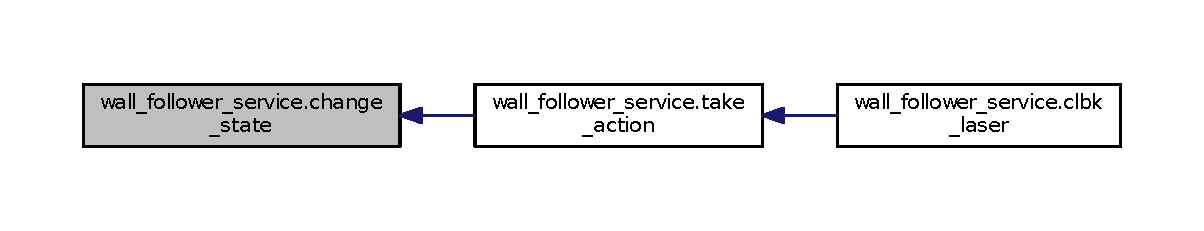
\includegraphics[width=350pt]{namespacewall__follower__service_a170c8a7e77b51a43f5b3edd8b0062ac4_icgraph}
\end{center}
\end{figure}


\index{wall\+\_\+follower\+\_\+service@{wall\+\_\+follower\+\_\+service}!clbk\+\_\+laser@{clbk\+\_\+laser}}
\index{clbk\+\_\+laser@{clbk\+\_\+laser}!wall\+\_\+follower\+\_\+service@{wall\+\_\+follower\+\_\+service}}
\subsubsection[{\texorpdfstring{clbk\+\_\+laser(msg)}{clbk_laser(msg)}}]{\setlength{\rightskip}{0pt plus 5cm}def wall\+\_\+follower\+\_\+service.\+clbk\+\_\+laser (
\begin{DoxyParamCaption}
\item[{}]{msg}
\end{DoxyParamCaption}
)}\hypertarget{namespacewall__follower__service_a09e3d81acac08943a5978c52bcbbfe26}{}\label{namespacewall__follower__service_a09e3d81acac08943a5978c52bcbbfe26}


Laser data callback output are localized in the robot in 5 regions organized as at the bottom. 

variable regions\+\_\+ separes the output of lasers 

Here is the call graph for this function\+:\nopagebreak
\begin{figure}[H]
\begin{center}
\leavevmode
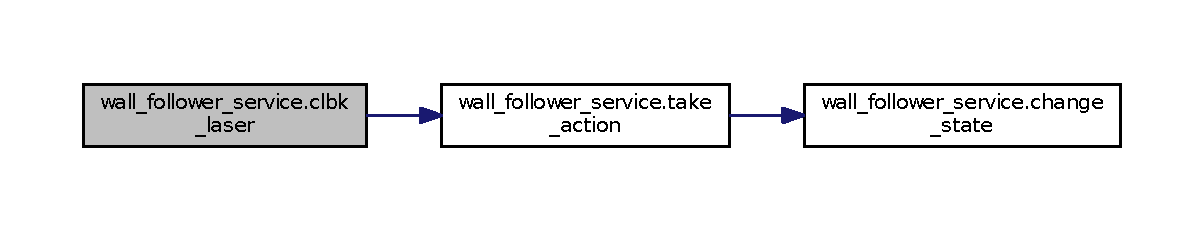
\includegraphics[width=350pt]{namespacewall__follower__service_a09e3d81acac08943a5978c52bcbbfe26_cgraph}
\end{center}
\end{figure}


\index{wall\+\_\+follower\+\_\+service@{wall\+\_\+follower\+\_\+service}!find\+\_\+wall@{find\+\_\+wall}}
\index{find\+\_\+wall@{find\+\_\+wall}!wall\+\_\+follower\+\_\+service@{wall\+\_\+follower\+\_\+service}}
\subsubsection[{\texorpdfstring{find\+\_\+wall()}{find_wall()}}]{\setlength{\rightskip}{0pt plus 5cm}def wall\+\_\+follower\+\_\+service.\+find\+\_\+wall (
\begin{DoxyParamCaption}
{}
\end{DoxyParamCaption}
)}\hypertarget{namespacewall__follower__service_a84de27c394cf900d7c30a6ab16409304}{}\label{namespacewall__follower__service_a84de27c394cf900d7c30a6ab16409304}


Function to find a wall. 

randomly searches for walls 

Here is the caller graph for this function\+:\nopagebreak
\begin{figure}[H]
\begin{center}
\leavevmode
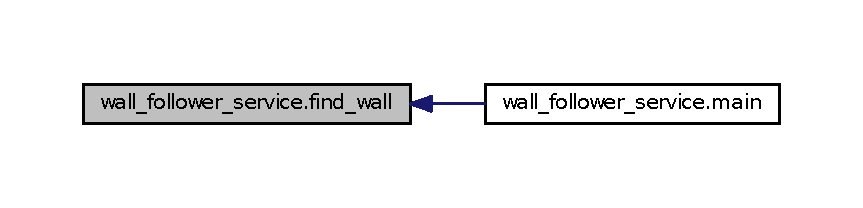
\includegraphics[width=350pt]{namespacewall__follower__service_a84de27c394cf900d7c30a6ab16409304_icgraph}
\end{center}
\end{figure}


\index{wall\+\_\+follower\+\_\+service@{wall\+\_\+follower\+\_\+service}!follow\+\_\+the\+\_\+wall@{follow\+\_\+the\+\_\+wall}}
\index{follow\+\_\+the\+\_\+wall@{follow\+\_\+the\+\_\+wall}!wall\+\_\+follower\+\_\+service@{wall\+\_\+follower\+\_\+service}}
\subsubsection[{\texorpdfstring{follow\+\_\+the\+\_\+wall()}{follow_the_wall()}}]{\setlength{\rightskip}{0pt plus 5cm}def wall\+\_\+follower\+\_\+service.\+follow\+\_\+the\+\_\+wall (
\begin{DoxyParamCaption}
{}
\end{DoxyParamCaption}
)}\hypertarget{namespacewall__follower__service_ac88d2c0d79a9b96805cd274c64d1bd80}{}\label{namespacewall__follower__service_ac88d2c0d79a9b96805cd274c64d1bd80}


Follow the wall function. 



Here is the caller graph for this function\+:\nopagebreak
\begin{figure}[H]
\begin{center}
\leavevmode
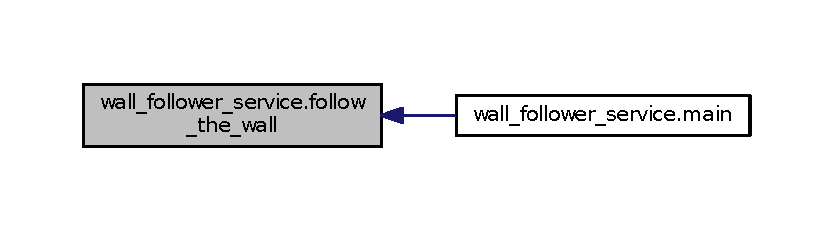
\includegraphics[width=350pt]{namespacewall__follower__service_ac88d2c0d79a9b96805cd274c64d1bd80_icgraph}
\end{center}
\end{figure}


\index{wall\+\_\+follower\+\_\+service@{wall\+\_\+follower\+\_\+service}!main@{main}}
\index{main@{main}!wall\+\_\+follower\+\_\+service@{wall\+\_\+follower\+\_\+service}}
\subsubsection[{\texorpdfstring{main()}{main()}}]{\setlength{\rightskip}{0pt plus 5cm}def wall\+\_\+follower\+\_\+service.\+main (
\begin{DoxyParamCaption}
{}
\end{DoxyParamCaption}
)}\hypertarget{namespacewall__follower__service_a91670567a06ba0f2b6d453eba9471c11}{}\label{namespacewall__follower__service_a91670567a06ba0f2b6d453eba9471c11}


Main function. 

initializes necessary variables, works as a state machine 

Here is the call graph for this function\+:\nopagebreak
\begin{figure}[H]
\begin{center}
\leavevmode
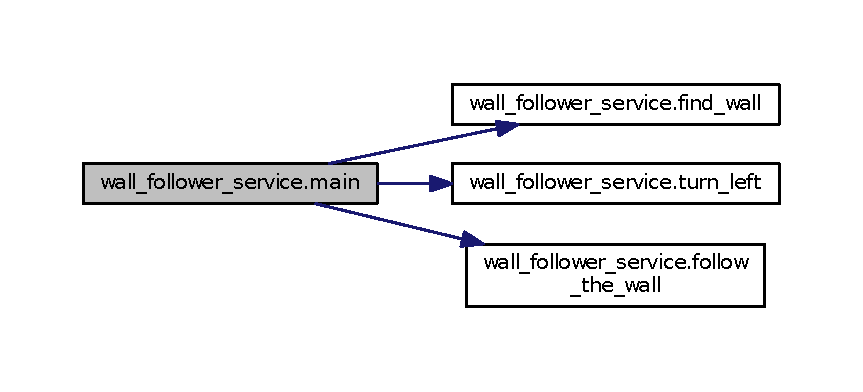
\includegraphics[width=350pt]{namespacewall__follower__service_a91670567a06ba0f2b6d453eba9471c11_cgraph}
\end{center}
\end{figure}


\index{wall\+\_\+follower\+\_\+service@{wall\+\_\+follower\+\_\+service}!take\+\_\+action@{take\+\_\+action}}
\index{take\+\_\+action@{take\+\_\+action}!wall\+\_\+follower\+\_\+service@{wall\+\_\+follower\+\_\+service}}
\subsubsection[{\texorpdfstring{take\+\_\+action()}{take_action()}}]{\setlength{\rightskip}{0pt plus 5cm}def wall\+\_\+follower\+\_\+service.\+take\+\_\+action (
\begin{DoxyParamCaption}
{}
\end{DoxyParamCaption}
)}\hypertarget{namespacewall__follower__service_a6627caa18de98475bf401975a5a4feb1}{}\label{namespacewall__follower__service_a6627caa18de98475bf401975a5a4feb1}


Take action function. 

checks the output of laser for knowing where are the position of wall with respect to oriantation and position of robot the robot change state according where wall are 

Here is the call graph for this function\+:\nopagebreak
\begin{figure}[H]
\begin{center}
\leavevmode
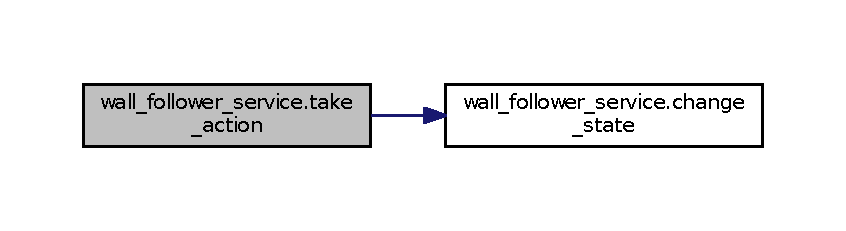
\includegraphics[width=350pt]{namespacewall__follower__service_a6627caa18de98475bf401975a5a4feb1_cgraph}
\end{center}
\end{figure}




Here is the caller graph for this function\+:\nopagebreak
\begin{figure}[H]
\begin{center}
\leavevmode
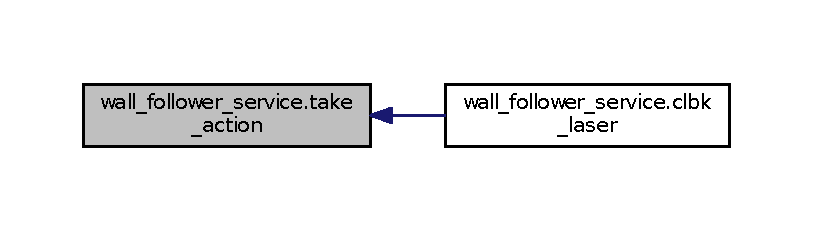
\includegraphics[width=350pt]{namespacewall__follower__service_a6627caa18de98475bf401975a5a4feb1_icgraph}
\end{center}
\end{figure}


\index{wall\+\_\+follower\+\_\+service@{wall\+\_\+follower\+\_\+service}!turn\+\_\+left@{turn\+\_\+left}}
\index{turn\+\_\+left@{turn\+\_\+left}!wall\+\_\+follower\+\_\+service@{wall\+\_\+follower\+\_\+service}}
\subsubsection[{\texorpdfstring{turn\+\_\+left()}{turn_left()}}]{\setlength{\rightskip}{0pt plus 5cm}def wall\+\_\+follower\+\_\+service.\+turn\+\_\+left (
\begin{DoxyParamCaption}
{}
\end{DoxyParamCaption}
)}\hypertarget{namespacewall__follower__service_a242dccb66f79027a138469906f3c10e1}{}\label{namespacewall__follower__service_a242dccb66f79027a138469906f3c10e1}


Turn left function. 



Here is the caller graph for this function\+:\nopagebreak
\begin{figure}[H]
\begin{center}
\leavevmode
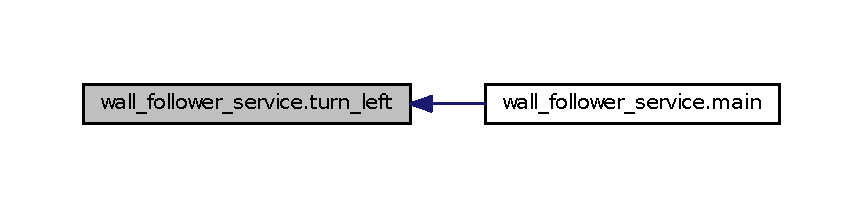
\includegraphics[width=350pt]{namespacewall__follower__service_a242dccb66f79027a138469906f3c10e1_icgraph}
\end{center}
\end{figure}


\index{wall\+\_\+follower\+\_\+service@{wall\+\_\+follower\+\_\+service}!wall\+\_\+follower\+\_\+switch@{wall\+\_\+follower\+\_\+switch}}
\index{wall\+\_\+follower\+\_\+switch@{wall\+\_\+follower\+\_\+switch}!wall\+\_\+follower\+\_\+service@{wall\+\_\+follower\+\_\+service}}
\subsubsection[{\texorpdfstring{wall\+\_\+follower\+\_\+switch(req)}{wall_follower_switch(req)}}]{\setlength{\rightskip}{0pt plus 5cm}def wall\+\_\+follower\+\_\+service.\+wall\+\_\+follower\+\_\+switch (
\begin{DoxyParamCaption}
\item[{}]{req}
\end{DoxyParamCaption}
)}\hypertarget{namespacewall__follower__service_a215aeb1ca629241f2f875ef081b21bb3}{}\label{namespacewall__follower__service_a215aeb1ca629241f2f875ef081b21bb3}


Function activated on service request. 


\begin{DoxyParams}{Parameters}
{\em req} & is the request of the service \\
\hline
\end{DoxyParams}


\subsection{Variable Documentation}
\index{wall\+\_\+follower\+\_\+service@{wall\+\_\+follower\+\_\+service}!active\+\_\+@{active\+\_\+}}
\index{active\+\_\+@{active\+\_\+}!wall\+\_\+follower\+\_\+service@{wall\+\_\+follower\+\_\+service}}
\subsubsection[{\texorpdfstring{active\+\_\+}{active_}}]{\setlength{\rightskip}{0pt plus 5cm}bool wall\+\_\+follower\+\_\+service.\+active\+\_\+ = False}\hypertarget{namespacewall__follower__service_acb03ef4ad62b64de43b4a4275d615e74}{}\label{namespacewall__follower__service_acb03ef4ad62b64de43b4a4275d615e74}
\index{wall\+\_\+follower\+\_\+service@{wall\+\_\+follower\+\_\+service}!pub\+\_\+@{pub\+\_\+}}
\index{pub\+\_\+@{pub\+\_\+}!wall\+\_\+follower\+\_\+service@{wall\+\_\+follower\+\_\+service}}
\subsubsection[{\texorpdfstring{pub\+\_\+}{pub_}}]{\setlength{\rightskip}{0pt plus 5cm}wall\+\_\+follower\+\_\+service.\+pub\+\_\+ = None}\hypertarget{namespacewall__follower__service_a2dba1ae8fd1b1af992b7872d2a7405f0}{}\label{namespacewall__follower__service_a2dba1ae8fd1b1af992b7872d2a7405f0}
\index{wall\+\_\+follower\+\_\+service@{wall\+\_\+follower\+\_\+service}!regions\+\_\+@{regions\+\_\+}}
\index{regions\+\_\+@{regions\+\_\+}!wall\+\_\+follower\+\_\+service@{wall\+\_\+follower\+\_\+service}}
\subsubsection[{\texorpdfstring{regions\+\_\+}{regions_}}]{\setlength{\rightskip}{0pt plus 5cm}dictionary wall\+\_\+follower\+\_\+service.\+regions\+\_\+}\hypertarget{namespacewall__follower__service_a5becd7ef6745adb020e646fde0af14f4}{}\label{namespacewall__follower__service_a5becd7ef6745adb020e646fde0af14f4}
{\bfseries Initial value\+:}
\begin{DoxyCode}
1 = \{
2     \textcolor{stringliteral}{'right'}: 0,
3     \textcolor{stringliteral}{'fright'}: 0,
4     \textcolor{stringliteral}{'front'}: 0,
5     \textcolor{stringliteral}{'fleft'}: 0,
6     \textcolor{stringliteral}{'left'}: 0,
7 \}
\end{DoxyCode}
\index{wall\+\_\+follower\+\_\+service@{wall\+\_\+follower\+\_\+service}!state\+\_\+@{state\+\_\+}}
\index{state\+\_\+@{state\+\_\+}!wall\+\_\+follower\+\_\+service@{wall\+\_\+follower\+\_\+service}}
\subsubsection[{\texorpdfstring{state\+\_\+}{state_}}]{\setlength{\rightskip}{0pt plus 5cm}int wall\+\_\+follower\+\_\+service.\+state\+\_\+ = 0}\hypertarget{namespacewall__follower__service_a85ced827917bea830636e97f3c2e737c}{}\label{namespacewall__follower__service_a85ced827917bea830636e97f3c2e737c}
\index{wall\+\_\+follower\+\_\+service@{wall\+\_\+follower\+\_\+service}!state\+\_\+dict\+\_\+@{state\+\_\+dict\+\_\+}}
\index{state\+\_\+dict\+\_\+@{state\+\_\+dict\+\_\+}!wall\+\_\+follower\+\_\+service@{wall\+\_\+follower\+\_\+service}}
\subsubsection[{\texorpdfstring{state\+\_\+dict\+\_\+}{state_dict_}}]{\setlength{\rightskip}{0pt plus 5cm}dictionary wall\+\_\+follower\+\_\+service.\+state\+\_\+dict\+\_\+}\hypertarget{namespacewall__follower__service_ad1235d309f9ac4c61a2c58c70b7e4895}{}\label{namespacewall__follower__service_ad1235d309f9ac4c61a2c58c70b7e4895}
{\bfseries Initial value\+:}
\begin{DoxyCode}
1 = \{
2     0: \textcolor{stringliteral}{'find the wall'},
3     1: \textcolor{stringliteral}{'turn left'},
4     2: \textcolor{stringliteral}{'follow the wall'},
5 \}
\end{DoxyCode}

\hypertarget{namespacewall__follower__service__bug}{}\section{wall\+\_\+follower\+\_\+service\+\_\+bug Namespace Reference}
\label{namespacewall__follower__service__bug}\index{wall\+\_\+follower\+\_\+service\+\_\+bug@{wall\+\_\+follower\+\_\+service\+\_\+bug}}
\subsection*{Functions}
\begin{DoxyCompactItemize}
\item 
def \hyperlink{namespacewall__follower__service__bug_a3d40480bf27a4e840ca68504fa2df3ab}{wall\+\_\+follower\+\_\+switch\+\_\+bug} (req)
\item 
def \hyperlink{namespacewall__follower__service__bug_a8b1d5bfaeda3631c84322d3139853b93}{clbk\+\_\+laser} (msg)
\item 
def \hyperlink{namespacewall__follower__service__bug_ad8938be3e565dc53359f86ffa73dc8ed}{change\+\_\+state} (state)
\item 
def \hyperlink{namespacewall__follower__service__bug_a6dca07c90a8a3a4108f601ede1e7332d}{take\+\_\+action} ()
\item 
def \hyperlink{namespacewall__follower__service__bug_ad7fc86411b01be176df591cf952867e7}{find\+\_\+wall} ()
\item 
def \hyperlink{namespacewall__follower__service__bug_a751a4853e801f3643502f84267a49713}{turn\+\_\+left} ()
\item 
def \hyperlink{namespacewall__follower__service__bug_aaf1e0a62c74840d77f6470c69efdc5fe}{follow\+\_\+the\+\_\+wall} ()
\item 
def \hyperlink{namespacewall__follower__service__bug_ac464970527026f0e4ab2086e8d0f9b09}{main} ()
\end{DoxyCompactItemize}
\subsection*{Variables}
\begin{DoxyCompactItemize}
\item 
bool \hyperlink{namespacewall__follower__service__bug_a2039142388607883c04a31004391c432}{active\+\_\+} = False
\item 
\hyperlink{namespacewall__follower__service__bug_a6a729bbbb58c90a8ad851df7cdb231eb}{pub\+\_\+} = None
\item 
dictionary \hyperlink{namespacewall__follower__service__bug_a17a692ba0d421dab426bc6232daed99e}{regions\+\_\+}
\item 
int \hyperlink{namespacewall__follower__service__bug_a96d928f6c8413cb0f1138c187ca0206a}{state\+\_\+} = 0
\item 
dictionary \hyperlink{namespacewall__follower__service__bug_a4559f30e607293b76c468006cf83eaa3}{state\+\_\+dict\+\_\+}
\end{DoxyCompactItemize}


\subsection{Function Documentation}
\index{wall\+\_\+follower\+\_\+service\+\_\+bug@{wall\+\_\+follower\+\_\+service\+\_\+bug}!change\+\_\+state@{change\+\_\+state}}
\index{change\+\_\+state@{change\+\_\+state}!wall\+\_\+follower\+\_\+service\+\_\+bug@{wall\+\_\+follower\+\_\+service\+\_\+bug}}
\subsubsection[{\texorpdfstring{change\+\_\+state(state)}{change_state(state)}}]{\setlength{\rightskip}{0pt plus 5cm}def wall\+\_\+follower\+\_\+service\+\_\+bug.\+change\+\_\+state (
\begin{DoxyParamCaption}
\item[{}]{state}
\end{DoxyParamCaption}
)}\hypertarget{namespacewall__follower__service__bug_ad8938be3e565dc53359f86ffa73dc8ed}{}\label{namespacewall__follower__service__bug_ad8938be3e565dc53359f86ffa73dc8ed}


Here is the caller graph for this function\+:\nopagebreak
\begin{figure}[H]
\begin{center}
\leavevmode
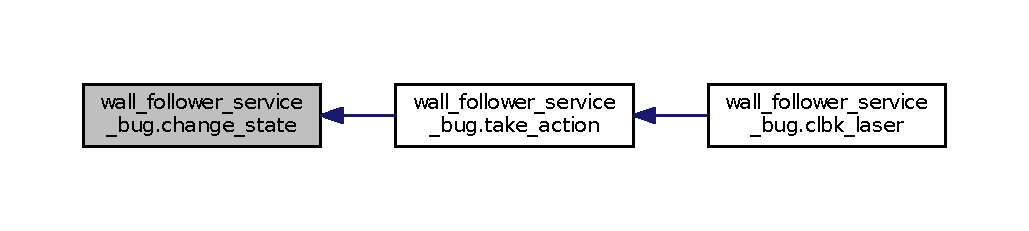
\includegraphics[width=350pt]{namespacewall__follower__service__bug_ad8938be3e565dc53359f86ffa73dc8ed_icgraph}
\end{center}
\end{figure}


\index{wall\+\_\+follower\+\_\+service\+\_\+bug@{wall\+\_\+follower\+\_\+service\+\_\+bug}!clbk\+\_\+laser@{clbk\+\_\+laser}}
\index{clbk\+\_\+laser@{clbk\+\_\+laser}!wall\+\_\+follower\+\_\+service\+\_\+bug@{wall\+\_\+follower\+\_\+service\+\_\+bug}}
\subsubsection[{\texorpdfstring{clbk\+\_\+laser(msg)}{clbk_laser(msg)}}]{\setlength{\rightskip}{0pt plus 5cm}def wall\+\_\+follower\+\_\+service\+\_\+bug.\+clbk\+\_\+laser (
\begin{DoxyParamCaption}
\item[{}]{msg}
\end{DoxyParamCaption}
)}\hypertarget{namespacewall__follower__service__bug_a8b1d5bfaeda3631c84322d3139853b93}{}\label{namespacewall__follower__service__bug_a8b1d5bfaeda3631c84322d3139853b93}


Here is the call graph for this function\+:\nopagebreak
\begin{figure}[H]
\begin{center}
\leavevmode
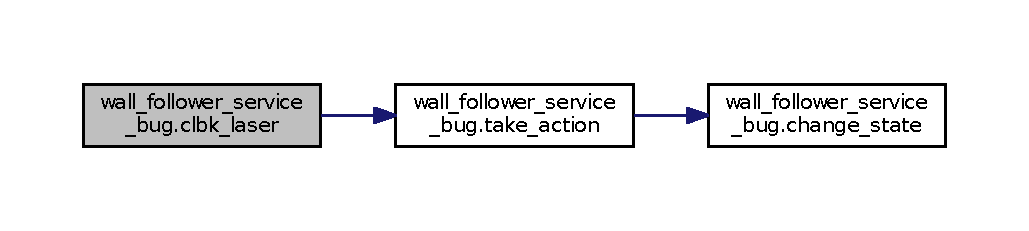
\includegraphics[width=350pt]{namespacewall__follower__service__bug_a8b1d5bfaeda3631c84322d3139853b93_cgraph}
\end{center}
\end{figure}


\index{wall\+\_\+follower\+\_\+service\+\_\+bug@{wall\+\_\+follower\+\_\+service\+\_\+bug}!find\+\_\+wall@{find\+\_\+wall}}
\index{find\+\_\+wall@{find\+\_\+wall}!wall\+\_\+follower\+\_\+service\+\_\+bug@{wall\+\_\+follower\+\_\+service\+\_\+bug}}
\subsubsection[{\texorpdfstring{find\+\_\+wall()}{find_wall()}}]{\setlength{\rightskip}{0pt plus 5cm}def wall\+\_\+follower\+\_\+service\+\_\+bug.\+find\+\_\+wall (
\begin{DoxyParamCaption}
{}
\end{DoxyParamCaption}
)}\hypertarget{namespacewall__follower__service__bug_ad7fc86411b01be176df591cf952867e7}{}\label{namespacewall__follower__service__bug_ad7fc86411b01be176df591cf952867e7}


Here is the caller graph for this function\+:\nopagebreak
\begin{figure}[H]
\begin{center}
\leavevmode
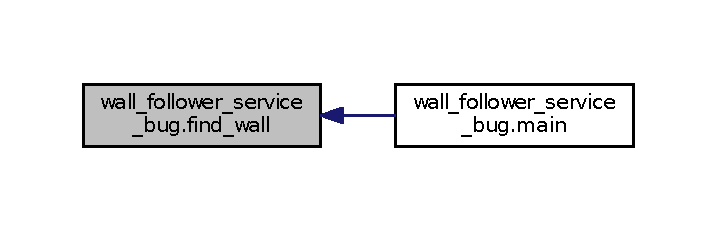
\includegraphics[width=344pt]{namespacewall__follower__service__bug_ad7fc86411b01be176df591cf952867e7_icgraph}
\end{center}
\end{figure}


\index{wall\+\_\+follower\+\_\+service\+\_\+bug@{wall\+\_\+follower\+\_\+service\+\_\+bug}!follow\+\_\+the\+\_\+wall@{follow\+\_\+the\+\_\+wall}}
\index{follow\+\_\+the\+\_\+wall@{follow\+\_\+the\+\_\+wall}!wall\+\_\+follower\+\_\+service\+\_\+bug@{wall\+\_\+follower\+\_\+service\+\_\+bug}}
\subsubsection[{\texorpdfstring{follow\+\_\+the\+\_\+wall()}{follow_the_wall()}}]{\setlength{\rightskip}{0pt plus 5cm}def wall\+\_\+follower\+\_\+service\+\_\+bug.\+follow\+\_\+the\+\_\+wall (
\begin{DoxyParamCaption}
{}
\end{DoxyParamCaption}
)}\hypertarget{namespacewall__follower__service__bug_aaf1e0a62c74840d77f6470c69efdc5fe}{}\label{namespacewall__follower__service__bug_aaf1e0a62c74840d77f6470c69efdc5fe}


Here is the caller graph for this function\+:\nopagebreak
\begin{figure}[H]
\begin{center}
\leavevmode
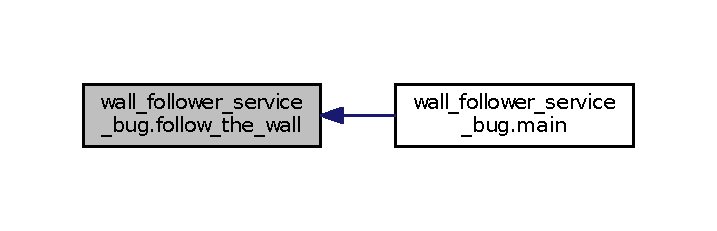
\includegraphics[width=344pt]{namespacewall__follower__service__bug_aaf1e0a62c74840d77f6470c69efdc5fe_icgraph}
\end{center}
\end{figure}


\index{wall\+\_\+follower\+\_\+service\+\_\+bug@{wall\+\_\+follower\+\_\+service\+\_\+bug}!main@{main}}
\index{main@{main}!wall\+\_\+follower\+\_\+service\+\_\+bug@{wall\+\_\+follower\+\_\+service\+\_\+bug}}
\subsubsection[{\texorpdfstring{main()}{main()}}]{\setlength{\rightskip}{0pt plus 5cm}def wall\+\_\+follower\+\_\+service\+\_\+bug.\+main (
\begin{DoxyParamCaption}
{}
\end{DoxyParamCaption}
)}\hypertarget{namespacewall__follower__service__bug_ac464970527026f0e4ab2086e8d0f9b09}{}\label{namespacewall__follower__service__bug_ac464970527026f0e4ab2086e8d0f9b09}


Here is the call graph for this function\+:\nopagebreak
\begin{figure}[H]
\begin{center}
\leavevmode
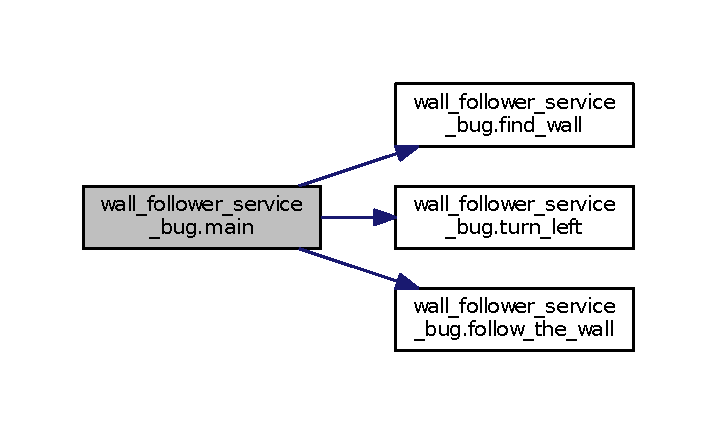
\includegraphics[width=344pt]{namespacewall__follower__service__bug_ac464970527026f0e4ab2086e8d0f9b09_cgraph}
\end{center}
\end{figure}


\index{wall\+\_\+follower\+\_\+service\+\_\+bug@{wall\+\_\+follower\+\_\+service\+\_\+bug}!take\+\_\+action@{take\+\_\+action}}
\index{take\+\_\+action@{take\+\_\+action}!wall\+\_\+follower\+\_\+service\+\_\+bug@{wall\+\_\+follower\+\_\+service\+\_\+bug}}
\subsubsection[{\texorpdfstring{take\+\_\+action()}{take_action()}}]{\setlength{\rightskip}{0pt plus 5cm}def wall\+\_\+follower\+\_\+service\+\_\+bug.\+take\+\_\+action (
\begin{DoxyParamCaption}
{}
\end{DoxyParamCaption}
)}\hypertarget{namespacewall__follower__service__bug_a6dca07c90a8a3a4108f601ede1e7332d}{}\label{namespacewall__follower__service__bug_a6dca07c90a8a3a4108f601ede1e7332d}


Here is the call graph for this function\+:\nopagebreak
\begin{figure}[H]
\begin{center}
\leavevmode
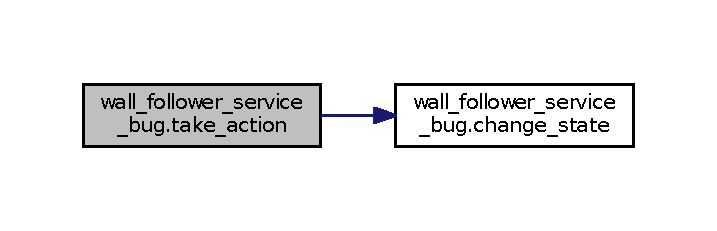
\includegraphics[width=344pt]{namespacewall__follower__service__bug_a6dca07c90a8a3a4108f601ede1e7332d_cgraph}
\end{center}
\end{figure}




Here is the caller graph for this function\+:\nopagebreak
\begin{figure}[H]
\begin{center}
\leavevmode
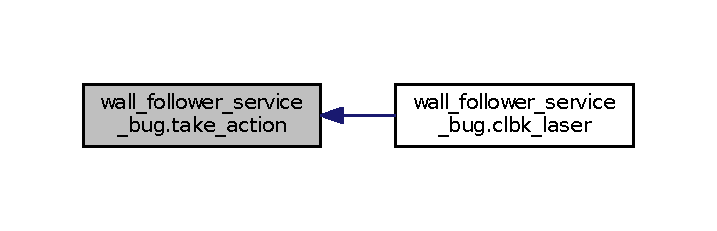
\includegraphics[width=344pt]{namespacewall__follower__service__bug_a6dca07c90a8a3a4108f601ede1e7332d_icgraph}
\end{center}
\end{figure}


\index{wall\+\_\+follower\+\_\+service\+\_\+bug@{wall\+\_\+follower\+\_\+service\+\_\+bug}!turn\+\_\+left@{turn\+\_\+left}}
\index{turn\+\_\+left@{turn\+\_\+left}!wall\+\_\+follower\+\_\+service\+\_\+bug@{wall\+\_\+follower\+\_\+service\+\_\+bug}}
\subsubsection[{\texorpdfstring{turn\+\_\+left()}{turn_left()}}]{\setlength{\rightskip}{0pt plus 5cm}def wall\+\_\+follower\+\_\+service\+\_\+bug.\+turn\+\_\+left (
\begin{DoxyParamCaption}
{}
\end{DoxyParamCaption}
)}\hypertarget{namespacewall__follower__service__bug_a751a4853e801f3643502f84267a49713}{}\label{namespacewall__follower__service__bug_a751a4853e801f3643502f84267a49713}


Here is the caller graph for this function\+:\nopagebreak
\begin{figure}[H]
\begin{center}
\leavevmode
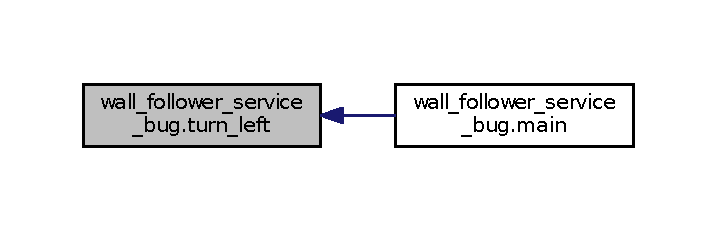
\includegraphics[width=344pt]{namespacewall__follower__service__bug_a751a4853e801f3643502f84267a49713_icgraph}
\end{center}
\end{figure}


\index{wall\+\_\+follower\+\_\+service\+\_\+bug@{wall\+\_\+follower\+\_\+service\+\_\+bug}!wall\+\_\+follower\+\_\+switch\+\_\+bug@{wall\+\_\+follower\+\_\+switch\+\_\+bug}}
\index{wall\+\_\+follower\+\_\+switch\+\_\+bug@{wall\+\_\+follower\+\_\+switch\+\_\+bug}!wall\+\_\+follower\+\_\+service\+\_\+bug@{wall\+\_\+follower\+\_\+service\+\_\+bug}}
\subsubsection[{\texorpdfstring{wall\+\_\+follower\+\_\+switch\+\_\+bug(req)}{wall_follower_switch_bug(req)}}]{\setlength{\rightskip}{0pt plus 5cm}def wall\+\_\+follower\+\_\+service\+\_\+bug.\+wall\+\_\+follower\+\_\+switch\+\_\+bug (
\begin{DoxyParamCaption}
\item[{}]{req}
\end{DoxyParamCaption}
)}\hypertarget{namespacewall__follower__service__bug_a3d40480bf27a4e840ca68504fa2df3ab}{}\label{namespacewall__follower__service__bug_a3d40480bf27a4e840ca68504fa2df3ab}


\subsection{Variable Documentation}
\index{wall\+\_\+follower\+\_\+service\+\_\+bug@{wall\+\_\+follower\+\_\+service\+\_\+bug}!active\+\_\+@{active\+\_\+}}
\index{active\+\_\+@{active\+\_\+}!wall\+\_\+follower\+\_\+service\+\_\+bug@{wall\+\_\+follower\+\_\+service\+\_\+bug}}
\subsubsection[{\texorpdfstring{active\+\_\+}{active_}}]{\setlength{\rightskip}{0pt plus 5cm}bool wall\+\_\+follower\+\_\+service\+\_\+bug.\+active\+\_\+ = False}\hypertarget{namespacewall__follower__service__bug_a2039142388607883c04a31004391c432}{}\label{namespacewall__follower__service__bug_a2039142388607883c04a31004391c432}
\index{wall\+\_\+follower\+\_\+service\+\_\+bug@{wall\+\_\+follower\+\_\+service\+\_\+bug}!pub\+\_\+@{pub\+\_\+}}
\index{pub\+\_\+@{pub\+\_\+}!wall\+\_\+follower\+\_\+service\+\_\+bug@{wall\+\_\+follower\+\_\+service\+\_\+bug}}
\subsubsection[{\texorpdfstring{pub\+\_\+}{pub_}}]{\setlength{\rightskip}{0pt plus 5cm}wall\+\_\+follower\+\_\+service\+\_\+bug.\+pub\+\_\+ = None}\hypertarget{namespacewall__follower__service__bug_a6a729bbbb58c90a8ad851df7cdb231eb}{}\label{namespacewall__follower__service__bug_a6a729bbbb58c90a8ad851df7cdb231eb}
\index{wall\+\_\+follower\+\_\+service\+\_\+bug@{wall\+\_\+follower\+\_\+service\+\_\+bug}!regions\+\_\+@{regions\+\_\+}}
\index{regions\+\_\+@{regions\+\_\+}!wall\+\_\+follower\+\_\+service\+\_\+bug@{wall\+\_\+follower\+\_\+service\+\_\+bug}}
\subsubsection[{\texorpdfstring{regions\+\_\+}{regions_}}]{\setlength{\rightskip}{0pt plus 5cm}dictionary wall\+\_\+follower\+\_\+service\+\_\+bug.\+regions\+\_\+}\hypertarget{namespacewall__follower__service__bug_a17a692ba0d421dab426bc6232daed99e}{}\label{namespacewall__follower__service__bug_a17a692ba0d421dab426bc6232daed99e}
{\bfseries Initial value\+:}
\begin{DoxyCode}
1 = \{
2     \textcolor{stringliteral}{'right'}: 0,
3     \textcolor{stringliteral}{'fright'}: 0,
4     \textcolor{stringliteral}{'front'}: 0,
5     \textcolor{stringliteral}{'fleft'}: 0,
6     \textcolor{stringliteral}{'left'}: 0,
7 \}
\end{DoxyCode}
\index{wall\+\_\+follower\+\_\+service\+\_\+bug@{wall\+\_\+follower\+\_\+service\+\_\+bug}!state\+\_\+@{state\+\_\+}}
\index{state\+\_\+@{state\+\_\+}!wall\+\_\+follower\+\_\+service\+\_\+bug@{wall\+\_\+follower\+\_\+service\+\_\+bug}}
\subsubsection[{\texorpdfstring{state\+\_\+}{state_}}]{\setlength{\rightskip}{0pt plus 5cm}int wall\+\_\+follower\+\_\+service\+\_\+bug.\+state\+\_\+ = 0}\hypertarget{namespacewall__follower__service__bug_a96d928f6c8413cb0f1138c187ca0206a}{}\label{namespacewall__follower__service__bug_a96d928f6c8413cb0f1138c187ca0206a}
\index{wall\+\_\+follower\+\_\+service\+\_\+bug@{wall\+\_\+follower\+\_\+service\+\_\+bug}!state\+\_\+dict\+\_\+@{state\+\_\+dict\+\_\+}}
\index{state\+\_\+dict\+\_\+@{state\+\_\+dict\+\_\+}!wall\+\_\+follower\+\_\+service\+\_\+bug@{wall\+\_\+follower\+\_\+service\+\_\+bug}}
\subsubsection[{\texorpdfstring{state\+\_\+dict\+\_\+}{state_dict_}}]{\setlength{\rightskip}{0pt plus 5cm}dictionary wall\+\_\+follower\+\_\+service\+\_\+bug.\+state\+\_\+dict\+\_\+}\hypertarget{namespacewall__follower__service__bug_a4559f30e607293b76c468006cf83eaa3}{}\label{namespacewall__follower__service__bug_a4559f30e607293b76c468006cf83eaa3}
{\bfseries Initial value\+:}
\begin{DoxyCode}
1 = \{
2     0: \textcolor{stringliteral}{'find the wall'},
3     1: \textcolor{stringliteral}{'turn left'},
4     2: \textcolor{stringliteral}{'follow the wall'},
5 \}
\end{DoxyCode}

\chapter{File Documentation}
\hypertarget{_r_e_a_d_m_e_8md}{}\section{R\+E\+A\+D\+M\+E.\+md File Reference}
\label{_r_e_a_d_m_e_8md}\index{R\+E\+A\+D\+M\+E.\+md@{R\+E\+A\+D\+M\+E.\+md}}

\hypertarget{big__brain_8py}{}\section{scripts/big\+\_\+brain.py File Reference}
\label{big__brain_8py}\index{scripts/big\+\_\+brain.\+py@{scripts/big\+\_\+brain.\+py}}
\subsection*{Namespaces}
\begin{DoxyCompactItemize}
\item 
 \hyperlink{namespacebig__brain}{big\+\_\+brain}
\item 
 \hyperlink{namespacefinal__assignment}{final\+\_\+assignment}
\begin{DoxyCompactList}\small\item\em This node is in charge of monitoring the state of the robot, and activate the corresping services and behaviour. \end{DoxyCompactList}\end{DoxyCompactItemize}
\subsection*{Functions}
\begin{DoxyCompactItemize}
\item 
def \hyperlink{namespacebig__brain_a815c120863ef1a5db7bf743bc9bb6f54}{big\+\_\+brain.\+clbk\+\_\+odom} (msg)
\begin{DoxyCompactList}\small\item\em Callback for keeping track of robot pose. \end{DoxyCompactList}\item 
def \hyperlink{namespacebig__brain_adfc26e0690fd9fe893e09be5400a8b7d}{big\+\_\+brain.\+distance} ()
\begin{DoxyCompactList}\small\item\em Function for computing the distance from the robot actual position to the desired position. \end{DoxyCompactList}\item 
def \hyperlink{namespacebig__brain_a4f091a106e4ba678afd9bc2df4f2789b}{big\+\_\+brain.\+new\+\_\+goal} ()
\begin{DoxyCompactList}\small\item\em Function for setting a new target with a Move\+Base\+Action\+Goal msg on topic /movebase/goal. \end{DoxyCompactList}\item 
def \hyperlink{namespacebig__brain_a108d0111d106a89cde8da1c2f494ab3c}{big\+\_\+brain.\+change\+\_\+state} (state)
\begin{DoxyCompactList}\small\item\em Function for changing the state of the robot. \end{DoxyCompactList}\item 
def \hyperlink{namespacebig__brain_a06516fa995f70f4013ee893ae15c5cea}{big\+\_\+brain.\+main} ()
\begin{DoxyCompactList}\small\item\em Main function. \end{DoxyCompactList}\end{DoxyCompactItemize}
\subsection*{Variables}
\begin{DoxyCompactItemize}
\item 
\hyperlink{namespacebig__brain_a9f12d1c3982160fe18122c7a2c4aa860}{big\+\_\+brain.\+twist\+\_\+pub} = None
\begin{DoxyCompactList}\small\item\em Publisher that publishes on /cmd\+\_\+vel to stop the robot when entering in state of \textquotesingle{}stop\textquotesingle{}. \end{DoxyCompactList}\item 
\hyperlink{namespacebig__brain_a757b56b184f850f2599be2279ac94777}{big\+\_\+brain.\+mvgoal\+\_\+pub} = None
\begin{DoxyCompactList}\small\item\em Publisher that publish a Move\+Base\+Action\+Goal msg on /move\+\_\+base/goal to make the robot reach the goal. \end{DoxyCompactList}\item 
\hyperlink{namespacebig__brain_acbbe2e86c0b737f0caaff69ce22b4aa8}{big\+\_\+brain.\+mvcancel\+\_\+pub} = None
\begin{DoxyCompactList}\small\item\em Publisher that publish a Goal\+ID msg on /move\+\_\+base/cancel to cancel a previous goal. \end{DoxyCompactList}\item 
\hyperlink{namespacebig__brain_a954157b5770aed51dc667611f39855b0}{big\+\_\+brain.\+srv\+\_\+client\+\_\+wall\+\_\+follower\+\_\+} = None
\begin{DoxyCompactList}\small\item\em Client for activating the service for wall following behaviour. \end{DoxyCompactList}\item 
\hyperlink{namespacebig__brain_a946162ac048b8df1f02003b37bd96812}{big\+\_\+brain.\+srv\+\_\+client\+\_\+user\+\_\+interface\+\_\+assignment\+\_\+} = None
\begin{DoxyCompactList}\small\item\em Client for activating the service calling the user main user interface. \end{DoxyCompactList}\item 
\hyperlink{namespacebig__brain_a60d3104e99b35d213a90529c7bc5a573}{big\+\_\+brain.\+srv\+\_\+client\+\_\+bug\+\_\+algorithm\+\_\+} = None
\begin{DoxyCompactList}\small\item\em C\+Lient for activating the bug navigation behaviour. \end{DoxyCompactList}\item 
\hyperlink{namespacebig__brain_a463bcdb8c7ed9954756492cdce9a43e2}{big\+\_\+brain.\+position\+\_\+} = Point()
\begin{DoxyCompactList}\small\item\em Variable containing position of the robot. \end{DoxyCompactList}\item 
\hyperlink{namespacebig__brain_a5f0f2fbee791fd60caa7a9dcf6ca1e00}{big\+\_\+brain.\+regions\+\_\+} = None
\begin{DoxyCompactList}\small\item\em Variables for controlling laser data. \end{DoxyCompactList}\item 
int \hyperlink{namespacebig__brain_ac43f9e8255d9b336a4f3ebe4dc3d2246}{big\+\_\+brain.\+change\+\_\+} = 0
\begin{DoxyCompactList}\small\item\em Variable for checking if a new state has been issued. \end{DoxyCompactList}\item 
list \hyperlink{namespacebig__brain_ab730e09c9bd7f5c7a1c09a8ea55a9029}{big\+\_\+brain.\+state\+\_\+desc\+\_\+} = \mbox{[}\textquotesingle{}random target\textquotesingle{}, \textquotesingle{}get target\textquotesingle{}, \textquotesingle{}wall fallowing\textquotesingle{},\textquotesingle{}stop\textquotesingle{},\textquotesingle{}bug\textquotesingle{}\mbox{]}
\begin{DoxyCompactList}\small\item\em States of the robot definiton. \end{DoxyCompactList}\item 
int \hyperlink{namespacebig__brain_a95db081b16847592a7981a7205e66358}{big\+\_\+brain.\+state\+\_\+} = 0
\begin{DoxyCompactList}\small\item\em Variable cointaining the actual state of the robot. \end{DoxyCompactList}\item 
int \hyperlink{namespacebig__brain_a28f405a0651539e59bd455a35ab07a3c}{big\+\_\+brain.\+newstate\+\_\+} = 0
\begin{DoxyCompactList}\small\item\em Variable containing the new state of the robot. \end{DoxyCompactList}\item 
int \hyperlink{namespacebig__brain_a82350019fe3047e74222abd0d6b07c14}{big\+\_\+brain.\+user\+\_\+} = 0
\begin{DoxyCompactList}\small\item\em Variable to control the different user interface when the behaviour is switched to bug. \end{DoxyCompactList}\end{DoxyCompactItemize}

\hypertarget{big__user__interface_8py}{}\section{scripts/big\+\_\+user\+\_\+interface.py File Reference}
\label{big__user__interface_8py}\index{scripts/big\+\_\+user\+\_\+interface.\+py@{scripts/big\+\_\+user\+\_\+interface.\+py}}
\subsection*{Namespaces}
\begin{DoxyCompactItemize}
\item 
 \hyperlink{namespacebig__user__interface}{big\+\_\+user\+\_\+interface}
\item 
 \hyperlink{namespacefinal__assignment}{final\+\_\+assignment}
\begin{DoxyCompactList}\small\item\em This node is in charge of monitoring the state of the robot, and activate the corresping services and behaviour. \end{DoxyCompactList}\end{DoxyCompactItemize}
\subsection*{Functions}
\begin{DoxyCompactItemize}
\item 
def \hyperlink{namespacebig__user__interface_a76119123837eb23b6351dfa51682c794}{big\+\_\+user\+\_\+interface.\+random\+\_\+trgt} (minimum, maximum)
\begin{DoxyCompactList}\small\item\em F\+Unction for setting a desired position. \end{DoxyCompactList}\item 
def \hyperlink{namespacebig__user__interface_a681a3a84ae63765bf0d5e1ea19486d57}{big\+\_\+user\+\_\+interface.\+assignment} (req)
\begin{DoxyCompactList}\small\item\em Function to assign a new behaviour to the robot. \end{DoxyCompactList}\item 
def \hyperlink{namespacebig__user__interface_ad2af43c69156cede1e27c973c8193d9c}{big\+\_\+user\+\_\+interface.\+main} ()
\begin{DoxyCompactList}\small\item\em Main function. \end{DoxyCompactList}\end{DoxyCompactItemize}

\hypertarget{bug__algo_8py}{}\section{scripts/bug\+\_\+algo.py File Reference}
\label{bug__algo_8py}\index{scripts/bug\+\_\+algo.\+py@{scripts/bug\+\_\+algo.\+py}}
\subsection*{Namespaces}
\begin{DoxyCompactItemize}
\item 
 \hyperlink{namespacebug__algo}{bug\+\_\+algo}
\item 
 \hyperlink{namespacefinal__assignment}{final\+\_\+assignment}
\begin{DoxyCompactList}\small\item\em This node is in charge of monitoring the state of the robot, and activate the corresping services and behaviour. \end{DoxyCompactList}\end{DoxyCompactItemize}
\subsection*{Functions}
\begin{DoxyCompactItemize}
\item 
def \hyperlink{namespacebug__algo_a6a72a118f8a289bf80b1fe79487b273f}{bug\+\_\+algo.\+clbk\+\_\+odom} (msg)
\begin{DoxyCompactList}\small\item\em Function to retrieve robot pose. \end{DoxyCompactList}\item 
def \hyperlink{namespacebug__algo_a4363ca4faa041280e958c5141bc3bde8}{bug\+\_\+algo.\+clbk\+\_\+laser} (msg)
\begin{DoxyCompactList}\small\item\em Laser data callback. \end{DoxyCompactList}\item 
def \hyperlink{namespacebug__algo_afe2965502b3ec1efdb6ac2dadfb9a5de}{bug\+\_\+algo.\+bug\+\_\+algorithm\+\_\+srv} (req)
\begin{DoxyCompactList}\small\item\em Function activated on service request. \end{DoxyCompactList}\item 
def \hyperlink{namespacebug__algo_aca287deda75aa8d0f790135ef47b6a16}{bug\+\_\+algo.\+change\+\_\+state} (state)
\begin{DoxyCompactList}\small\item\em Change state function. \end{DoxyCompactList}\item 
def \hyperlink{namespacebug__algo_ae499da57d8d88a30b64054480fdb60c8}{bug\+\_\+algo.\+normalize\+\_\+angle} (angle)
\begin{DoxyCompactList}\small\item\em Normalize angle function. \end{DoxyCompactList}\item 
def \hyperlink{namespacebug__algo_a8df2ef2049aa935d5478597523b50dcb}{bug\+\_\+algo.\+main} ()
\begin{DoxyCompactList}\small\item\em Main function. \end{DoxyCompactList}\end{DoxyCompactItemize}
\subsection*{Variables}
\begin{DoxyCompactItemize}
\item 
bool \hyperlink{namespacebug__algo_a3bec537d2bfc115b0a14ee6bad41bd00}{bug\+\_\+algo.\+active\+\_\+} = False
\item 
int \hyperlink{namespacebug__algo_a6ff626c7bf6a4dfec4e8508d8ae5097c}{bug\+\_\+algo.\+start\+\_\+time} = 0
\item 
int \hyperlink{namespacebug__algo_af723ba0d909555b34934483c74e06818}{bug\+\_\+algo.\+elapsed\+\_\+time} = 0
\item 
int \hyperlink{namespacebug__algo_af9e77fe7842316d1491ef585c7602710}{bug\+\_\+algo.\+actual\+\_\+time} = 0
\item 
\hyperlink{namespacebug__algo_a17a7504f2f0f6714f6ac31a43107fc31}{bug\+\_\+algo.\+pub} = None
\item 
\hyperlink{namespacebug__algo_a52e8d210b667d955534f12f59f191eb3}{bug\+\_\+algo.\+srv\+\_\+client\+\_\+go\+\_\+to\+\_\+point\+\_\+} = None
\item 
\hyperlink{namespacebug__algo_afe0f6c6a1a9bc751e4bbcae499815585}{bug\+\_\+algo.\+srv\+\_\+client\+\_\+wall\+\_\+follower\+\_\+} = None
\item 
\hyperlink{namespacebug__algo_a1a55011236874d9af4afcf4c3524bbf0}{bug\+\_\+algo.\+srv\+\_\+client\+\_\+user\+\_\+interface\+\_\+} = None
\item 
\hyperlink{namespacebug__algo_ac9de3b470960260c4510748850446480}{bug\+\_\+algo.\+srv\+\_\+client\+\_\+user\+\_\+interface\+\_\+assignment\+\_\+} = None
\item 
int \hyperlink{namespacebug__algo_a2c8d86dd369e86415dc7ff9c617033d7}{bug\+\_\+algo.\+yaw\+\_\+} = 0
\item 
int \hyperlink{namespacebug__algo_a3714c955ff3cf688c84d6dc5654833d6}{bug\+\_\+algo.\+yaw\+\_\+error\+\_\+allowed\+\_\+} = 5
\item 
\hyperlink{namespacebug__algo_ac0035ad008802f966f437b4787365220}{bug\+\_\+algo.\+position\+\_\+} = Point()
\item 
\hyperlink{namespacebug__algo_a6bc76d9dd5213819c8287c8833f8f3bd}{bug\+\_\+algo.\+desired\+\_\+position\+\_\+} = Point()
\item 
\hyperlink{namespacebug__algo_ae006850add8691db5d752b4ccb732ac1}{bug\+\_\+algo.\+x}
\item 
\hyperlink{namespacebug__algo_a1e2d049a4b898c92454f0fb146a413ee}{bug\+\_\+algo.\+y}
\item 
\hyperlink{namespacebug__algo_ad9944dcf5037184fbfbe3162935d2a57}{bug\+\_\+algo.\+z}
\item 
\hyperlink{namespacebug__algo_a31fd6300649f8a600eb87ebed00b174f}{bug\+\_\+algo.\+regions\+\_\+} = None
\item 
list \hyperlink{namespacebug__algo_a419cb7998b9a3946692fc01f5d73a25b}{bug\+\_\+algo.\+state\+\_\+desc\+\_\+} = \mbox{[}\textquotesingle{}Go to point\textquotesingle{}, \textquotesingle{}wall following\textquotesingle{}, \textquotesingle{}stopped\textquotesingle{}\mbox{]}
\item 
int \hyperlink{namespacebug__algo_a5bf52a66b7821a097f6e653a2422748e}{bug\+\_\+algo.\+state\+\_\+} = 0
\end{DoxyCompactItemize}

\hypertarget{go__to__point__service__bug_8py}{}\section{scripts/go\+\_\+to\+\_\+point\+\_\+service\+\_\+bug.py File Reference}
\label{go__to__point__service__bug_8py}\index{scripts/go\+\_\+to\+\_\+point\+\_\+service\+\_\+bug.\+py@{scripts/go\+\_\+to\+\_\+point\+\_\+service\+\_\+bug.\+py}}
\subsection*{Namespaces}
\begin{DoxyCompactItemize}
\item 
 \hyperlink{namespacego__to__point__service__bug}{go\+\_\+to\+\_\+point\+\_\+service\+\_\+bug}
\item 
 \hyperlink{namespacefinal__assignment}{final\+\_\+assignment}
\begin{DoxyCompactList}\small\item\em This node is in charge of monitoring the state of the robot, and activate the corresping services and behaviour. \end{DoxyCompactList}\end{DoxyCompactItemize}
\subsection*{Functions}
\begin{DoxyCompactItemize}
\item 
def \hyperlink{namespacego__to__point__service__bug_a66835918820d392cf39cc1e3b28497ee}{go\+\_\+to\+\_\+point\+\_\+service\+\_\+bug.\+go\+\_\+to\+\_\+point\+\_\+switch} (req)
\begin{DoxyCompactList}\small\item\em Function activated on service request. \end{DoxyCompactList}\item 
def \hyperlink{namespacego__to__point__service__bug_acc2367a3fc6946e8ea518d82a018dcd7}{go\+\_\+to\+\_\+point\+\_\+service\+\_\+bug.\+clbk\+\_\+odom} (msg)
\begin{DoxyCompactList}\small\item\em Function to retrieve robot pose. \end{DoxyCompactList}\item 
def \hyperlink{namespacego__to__point__service__bug_a99587ca3714f1c59523a0fccdb4acc7d}{go\+\_\+to\+\_\+point\+\_\+service\+\_\+bug.\+change\+\_\+state} (state)
\begin{DoxyCompactList}\small\item\em Change state function. \end{DoxyCompactList}\item 
def \hyperlink{namespacego__to__point__service__bug_a3ff83aec5e0de49fa33f2d33681d2a49}{go\+\_\+to\+\_\+point\+\_\+service\+\_\+bug.\+normalize\+\_\+angle} (angle)
\begin{DoxyCompactList}\small\item\em Normalize angle function. \end{DoxyCompactList}\item 
def \hyperlink{namespacego__to__point__service__bug_a0f4f965c49e3e20c6442b10bf41e2533}{go\+\_\+to\+\_\+point\+\_\+service\+\_\+bug.\+fix\+\_\+yaw} (des\+\_\+pos)
\begin{DoxyCompactList}\small\item\em Fix Yah function. \end{DoxyCompactList}\item 
def \hyperlink{namespacego__to__point__service__bug_a78a4659fd178f90a4b0acb3a4da0fbc1}{go\+\_\+to\+\_\+point\+\_\+service\+\_\+bug.\+go\+\_\+straight\+\_\+ahead} (des\+\_\+pos)
\begin{DoxyCompactList}\small\item\em Go straight function. \end{DoxyCompactList}\item 
def \hyperlink{namespacego__to__point__service__bug_a181271bc83dc620614c43e6bd6b18db8}{go\+\_\+to\+\_\+point\+\_\+service\+\_\+bug.\+done} (des\+\_\+pos)
\begin{DoxyCompactList}\small\item\em Done function. \end{DoxyCompactList}\item 
def \hyperlink{namespacego__to__point__service__bug_abb5a5a69905cef8ab5baf0768056ecea}{go\+\_\+to\+\_\+point\+\_\+service\+\_\+bug.\+main} ()
\begin{DoxyCompactList}\small\item\em Main function. \end{DoxyCompactList}\end{DoxyCompactItemize}
\subsection*{Variables}
\begin{DoxyCompactItemize}
\item 
bool \hyperlink{namespacego__to__point__service__bug_a904337d36bd7e3e63dc3d862b0f67608}{go\+\_\+to\+\_\+point\+\_\+service\+\_\+bug.\+active\+\_\+} = False
\item 
\hyperlink{namespacego__to__point__service__bug_a8eccd57782f5a63758c2ed6fc429648f}{go\+\_\+to\+\_\+point\+\_\+service\+\_\+bug.\+position\+\_\+} = Point()
\item 
int \hyperlink{namespacego__to__point__service__bug_a92ae1b18b13762d59aa27dd83ea9e04d}{go\+\_\+to\+\_\+point\+\_\+service\+\_\+bug.\+yaw\+\_\+} = 0
\item 
int \hyperlink{namespacego__to__point__service__bug_acf82697453e220209d6f386e1630619a}{go\+\_\+to\+\_\+point\+\_\+service\+\_\+bug.\+state\+\_\+} = 0
\item 
\hyperlink{namespacego__to__point__service__bug_a5c33b74b7f2376e73690f8474fc4db36}{go\+\_\+to\+\_\+point\+\_\+service\+\_\+bug.\+desired\+\_\+position\+\_\+} = Point()
\item 
\hyperlink{namespacego__to__point__service__bug_a6761dc57b29d40d3e6578b775a1e84c2}{go\+\_\+to\+\_\+point\+\_\+service\+\_\+bug.\+x}
\item 
\hyperlink{namespacego__to__point__service__bug_a9eac097a440f4f16c9e7260e5296fd76}{go\+\_\+to\+\_\+point\+\_\+service\+\_\+bug.\+y}
\item 
\hyperlink{namespacego__to__point__service__bug_ac72a9ad64f48ea907c94e25a3718372c}{go\+\_\+to\+\_\+point\+\_\+service\+\_\+bug.\+z}
\item 
int \hyperlink{namespacego__to__point__service__bug_aa27745ad563c25adbac628695bbdd44d}{go\+\_\+to\+\_\+point\+\_\+service\+\_\+bug.\+yaw\+\_\+precision\+\_\+} = math.\+pi/9
\item 
int \hyperlink{namespacego__to__point__service__bug_a2cfb8eb9d839627bee23494c162a1e88}{go\+\_\+to\+\_\+point\+\_\+service\+\_\+bug.\+yaw\+\_\+precision\+\_\+2\+\_\+} = math.\+pi/90
\item 
float \hyperlink{namespacego__to__point__service__bug_a1142014aa3b5c0819cd183c7b4534927}{go\+\_\+to\+\_\+point\+\_\+service\+\_\+bug.\+dist\+\_\+precision\+\_\+} = 0.\+3
\item 
float \hyperlink{namespacego__to__point__service__bug_ab4d1411316c963d5b211e42f78cf3c93}{go\+\_\+to\+\_\+point\+\_\+service\+\_\+bug.\+kp\+\_\+a} = 3.\+0
\item 
float \hyperlink{namespacego__to__point__service__bug_a0aa73d2814be9d22fc2a6e4eaa0afc07}{go\+\_\+to\+\_\+point\+\_\+service\+\_\+bug.\+kp\+\_\+d} = 0.\+2
\item 
float \hyperlink{namespacego__to__point__service__bug_aa2cfb37c171e32902af10e4f4121f92f}{go\+\_\+to\+\_\+point\+\_\+service\+\_\+bug.\+ub\+\_\+a} = 0.\+6
\item 
float \hyperlink{namespacego__to__point__service__bug_a60404a026e5fcd840f8a6f712edfb71f}{go\+\_\+to\+\_\+point\+\_\+service\+\_\+bug.\+lb\+\_\+a} = -\/0.\+5
\item 
float \hyperlink{namespacego__to__point__service__bug_a0ea364ac6b209e590e96109ca6fb7a5c}{go\+\_\+to\+\_\+point\+\_\+service\+\_\+bug.\+ub\+\_\+d} = 0.\+6
\item 
\hyperlink{namespacego__to__point__service__bug_a303812c1ccf752e711d273e93c27293d}{go\+\_\+to\+\_\+point\+\_\+service\+\_\+bug.\+pub} = None
\end{DoxyCompactItemize}

\hypertarget{user__interface_8py}{}\section{scripts/user\+\_\+interface.py File Reference}
\label{user__interface_8py}\index{scripts/user\+\_\+interface.\+py@{scripts/user\+\_\+interface.\+py}}
\subsection*{Namespaces}
\begin{DoxyCompactItemize}
\item 
 \hyperlink{namespaceuser__interface}{user\+\_\+interface}
\item 
 \hyperlink{namespacefinal__assignment}{final\+\_\+assignment}
\begin{DoxyCompactList}\small\item\em This node is in charge of monitoring the state of the robot, and activate the corresping services and behaviour. \end{DoxyCompactList}\end{DoxyCompactItemize}
\subsection*{Functions}
\begin{DoxyCompactItemize}
\item 
def \hyperlink{namespaceuser__interface_aa9dc3b0346ac037400ae347eb6efb788}{user\+\_\+interface.\+set\+\_\+new\+\_\+pos} (req)
\begin{DoxyCompactList}\small\item\em Function to set the new position for bug algoritm. \end{DoxyCompactList}\item 
def \hyperlink{namespaceuser__interface_ac26bdb296b6776907b72c17ce5a1b24a}{user\+\_\+interface.\+main} ()
\begin{DoxyCompactList}\small\item\em Main function. \end{DoxyCompactList}\end{DoxyCompactItemize}

\hypertarget{wall__follower__service_8py}{}\section{scripts/wall\+\_\+follower\+\_\+service.py File Reference}
\label{wall__follower__service_8py}\index{scripts/wall\+\_\+follower\+\_\+service.\+py@{scripts/wall\+\_\+follower\+\_\+service.\+py}}
\subsection*{Namespaces}
\begin{DoxyCompactItemize}
\item 
 \hyperlink{namespacewall__follower__service}{wall\+\_\+follower\+\_\+service}
\item 
 \hyperlink{namespacefinal__assignment}{final\+\_\+assignment}
\begin{DoxyCompactList}\small\item\em This node is in charge of monitoring the state of the robot, and activate the corresping services and behaviour. \end{DoxyCompactList}\end{DoxyCompactItemize}
\subsection*{Functions}
\begin{DoxyCompactItemize}
\item 
def \hyperlink{namespacewall__follower__service_a215aeb1ca629241f2f875ef081b21bb3}{wall\+\_\+follower\+\_\+service.\+wall\+\_\+follower\+\_\+switch} (req)
\begin{DoxyCompactList}\small\item\em Function activated on service request. \end{DoxyCompactList}\item 
def \hyperlink{namespacewall__follower__service_a09e3d81acac08943a5978c52bcbbfe26}{wall\+\_\+follower\+\_\+service.\+clbk\+\_\+laser} (msg)
\begin{DoxyCompactList}\small\item\em Laser data callback output are localized in the robot in 5 regions organized as at the bottom. \end{DoxyCompactList}\item 
def \hyperlink{namespacewall__follower__service_a170c8a7e77b51a43f5b3edd8b0062ac4}{wall\+\_\+follower\+\_\+service.\+change\+\_\+state} (state)
\begin{DoxyCompactList}\small\item\em Change state function. \end{DoxyCompactList}\item 
def \hyperlink{namespacewall__follower__service_a6627caa18de98475bf401975a5a4feb1}{wall\+\_\+follower\+\_\+service.\+take\+\_\+action} ()
\begin{DoxyCompactList}\small\item\em Take action function. \end{DoxyCompactList}\item 
def \hyperlink{namespacewall__follower__service_a84de27c394cf900d7c30a6ab16409304}{wall\+\_\+follower\+\_\+service.\+find\+\_\+wall} ()
\begin{DoxyCompactList}\small\item\em Function to find a wall. \end{DoxyCompactList}\item 
def \hyperlink{namespacewall__follower__service_a242dccb66f79027a138469906f3c10e1}{wall\+\_\+follower\+\_\+service.\+turn\+\_\+left} ()
\begin{DoxyCompactList}\small\item\em Turn left function. \end{DoxyCompactList}\item 
def \hyperlink{namespacewall__follower__service_ac88d2c0d79a9b96805cd274c64d1bd80}{wall\+\_\+follower\+\_\+service.\+follow\+\_\+the\+\_\+wall} ()
\begin{DoxyCompactList}\small\item\em Follow the wall function. \end{DoxyCompactList}\item 
def \hyperlink{namespacewall__follower__service_a91670567a06ba0f2b6d453eba9471c11}{wall\+\_\+follower\+\_\+service.\+main} ()
\begin{DoxyCompactList}\small\item\em Main function. \end{DoxyCompactList}\end{DoxyCompactItemize}
\subsection*{Variables}
\begin{DoxyCompactItemize}
\item 
bool \hyperlink{namespacewall__follower__service_acb03ef4ad62b64de43b4a4275d615e74}{wall\+\_\+follower\+\_\+service.\+active\+\_\+} = False
\item 
\hyperlink{namespacewall__follower__service_a2dba1ae8fd1b1af992b7872d2a7405f0}{wall\+\_\+follower\+\_\+service.\+pub\+\_\+} = None
\item 
dictionary \hyperlink{namespacewall__follower__service_a5becd7ef6745adb020e646fde0af14f4}{wall\+\_\+follower\+\_\+service.\+regions\+\_\+}
\item 
int \hyperlink{namespacewall__follower__service_a85ced827917bea830636e97f3c2e737c}{wall\+\_\+follower\+\_\+service.\+state\+\_\+} = 0
\item 
dictionary \hyperlink{namespacewall__follower__service_ad1235d309f9ac4c61a2c58c70b7e4895}{wall\+\_\+follower\+\_\+service.\+state\+\_\+dict\+\_\+}
\end{DoxyCompactItemize}

\hypertarget{wall__follower__service__bug_8py}{}\section{scripts/wall\+\_\+follower\+\_\+service\+\_\+bug.py File Reference}
\label{wall__follower__service__bug_8py}\index{scripts/wall\+\_\+follower\+\_\+service\+\_\+bug.\+py@{scripts/wall\+\_\+follower\+\_\+service\+\_\+bug.\+py}}
\subsection*{Namespaces}
\begin{DoxyCompactItemize}
\item 
 \hyperlink{namespacewall__follower__service__bug}{wall\+\_\+follower\+\_\+service\+\_\+bug}
\item 
 \hyperlink{namespacefinal__assignment}{final\+\_\+assignment}
\begin{DoxyCompactList}\small\item\em This node is in charge of monitoring the state of the robot, and activate the corresping services and behaviour. \end{DoxyCompactList}\end{DoxyCompactItemize}
\subsection*{Functions}
\begin{DoxyCompactItemize}
\item 
def \hyperlink{namespacewall__follower__service__bug_a3d40480bf27a4e840ca68504fa2df3ab}{wall\+\_\+follower\+\_\+service\+\_\+bug.\+wall\+\_\+follower\+\_\+switch\+\_\+bug} (req)
\item 
def \hyperlink{namespacewall__follower__service__bug_a8b1d5bfaeda3631c84322d3139853b93}{wall\+\_\+follower\+\_\+service\+\_\+bug.\+clbk\+\_\+laser} (msg)
\item 
def \hyperlink{namespacewall__follower__service__bug_ad8938be3e565dc53359f86ffa73dc8ed}{wall\+\_\+follower\+\_\+service\+\_\+bug.\+change\+\_\+state} (state)
\item 
def \hyperlink{namespacewall__follower__service__bug_a6dca07c90a8a3a4108f601ede1e7332d}{wall\+\_\+follower\+\_\+service\+\_\+bug.\+take\+\_\+action} ()
\item 
def \hyperlink{namespacewall__follower__service__bug_ad7fc86411b01be176df591cf952867e7}{wall\+\_\+follower\+\_\+service\+\_\+bug.\+find\+\_\+wall} ()
\item 
def \hyperlink{namespacewall__follower__service__bug_a751a4853e801f3643502f84267a49713}{wall\+\_\+follower\+\_\+service\+\_\+bug.\+turn\+\_\+left} ()
\item 
def \hyperlink{namespacewall__follower__service__bug_aaf1e0a62c74840d77f6470c69efdc5fe}{wall\+\_\+follower\+\_\+service\+\_\+bug.\+follow\+\_\+the\+\_\+wall} ()
\item 
def \hyperlink{namespacewall__follower__service__bug_ac464970527026f0e4ab2086e8d0f9b09}{wall\+\_\+follower\+\_\+service\+\_\+bug.\+main} ()
\end{DoxyCompactItemize}
\subsection*{Variables}
\begin{DoxyCompactItemize}
\item 
bool \hyperlink{namespacewall__follower__service__bug_a2039142388607883c04a31004391c432}{wall\+\_\+follower\+\_\+service\+\_\+bug.\+active\+\_\+} = False
\item 
\hyperlink{namespacewall__follower__service__bug_a6a729bbbb58c90a8ad851df7cdb231eb}{wall\+\_\+follower\+\_\+service\+\_\+bug.\+pub\+\_\+} = None
\item 
dictionary \hyperlink{namespacewall__follower__service__bug_a17a692ba0d421dab426bc6232daed99e}{wall\+\_\+follower\+\_\+service\+\_\+bug.\+regions\+\_\+}
\item 
int \hyperlink{namespacewall__follower__service__bug_a96d928f6c8413cb0f1138c187ca0206a}{wall\+\_\+follower\+\_\+service\+\_\+bug.\+state\+\_\+} = 0
\item 
dictionary \hyperlink{namespacewall__follower__service__bug_a4559f30e607293b76c468006cf83eaa3}{wall\+\_\+follower\+\_\+service\+\_\+bug.\+state\+\_\+dict\+\_\+}
\end{DoxyCompactItemize}

%--- End generated contents ---

% Index
\backmatter
\newpage
\phantomsection
\clearemptydoublepage
\addcontentsline{toc}{chapter}{Index}
\printindex

\end{document}
